
\documentclass{beamer}
\usepackage{graphicx}
\usepackage[super]{nth}
\usetheme{Malmoe}
\newcommand{\ts}{\textsuperscript}

\makeatletter
    \newenvironment{withoutheadline}{
        \setbeamertemplate{headline}[default]
        \def\beamer@entrycode{\vspace*{-\headheight}}
    }{}
\makeatother


\beamertemplatenavigationsymbolsempty
\makeatother
\setbeamertemplate{footline}
{
  \leavevmode%
  \hbox{%
  \begin{beamercolorbox}[wd=.4\paperwidth,ht=2.25ex,dp=1ex,center]{author in head/foot}%
    \usebeamerfont{author in head/foot}\insertshortauthor
  \end{beamercolorbox}%
  \begin{beamercolorbox}[wd=.6\paperwidth,ht=2.25ex,dp=1ex,center]{title in head/foot}%
    \usebeamerfont{title in head/foot}\insertshorttitle\hspace*{3em}
    \insertframenumber{} / 19
  \end{beamercolorbox}}%
  \vskip0pt%
}
%%%%%%%%%%FIRST SLIDE%%%%%%%%%%

\setbeamercolor*{title}{use=structure,fg=white,bg=structure.fg}
\setbeamertemplate{title page}[default][colsep=-4bp,rounded=true,shadow=true]
\title[Collision Prevention in Distributed 6TiSCH Networks]{Collision Prevention \\in Distributed 6TiSCH Networks}

\author{ Ali Jawad Fahs\\}


\institute[Universities of Somewhere and Elsewhere] 
{Universit\'e Grenoble Alpes (UGA) - UFR IM\textsuperscript{2}AG \\
Grenoble INP - Ensimag\\
Laboratoire d'Informatique de Grenoble (LIG), Team Drakkar \\
VERIMAG, Synchrone\\
\vskip 1em
Authors: Ali J. Fahs, Rodolphe Bertolini  \\ Dr. Olivier Alphand, Dr. Franck Rousseau \\
 Dr. Karine Altisen, Dr. St\'ephane Devismes \\

 }

\date{WiMob 2017, \nth{10} of October,2017}


\subject{Wireless Sensor Networks}
%%%%%%%%%%%%%%%%%%%%%%%% OUTLINE%%%%%%%%%%%%
\AtBeginSubsection[]
{ \begin{withoutheadline}
\setbeamertemplate{footline}{} 
  \begin{frame}<beamer>{Outline}
  
    \tableofcontents[currentsection,currentsubsection]
  \end{frame}
  \end{withoutheadline}
}

%%%%%%%%%%%%%%%%%%%% SLIDES %%%%%%%%%%%%%%%%




\begin{document}
\begin{withoutheadline}
\setbeamertemplate{footline}{} 
\begin{frame}
  \titlepage

\begin{itemize}
\item[]
\begin{center}


\includegraphics[width=0.13\linewidth]{figures/logo_im2ag_h122.jpg} \hskip 1em

\includegraphics[width=0.16\linewidth]{figures/Logo_ENSIMAG_2008-svg.png} \hskip 1em

\includegraphics[width=0.135\linewidth]{figures/LIG_test.png}  \hskip 1em

\includegraphics[width=0.14\linewidth]{figures/verimag.jpg}
\end{center}
\end{itemize}


\end{frame}

%%%%%%%%%%%%%%%%%%%%%%%% first %%%%%%%%%%%%%%%%%%%%%
\end{withoutheadline}

\begin{withoutheadline}
    \begin{frame}{Outline} % and our simple frame
        \tableofcontents
        \addtocounter{framenumber}{-1}
    \end{frame}
\end{withoutheadline}
%%%%%%%%%%%%%%%%%%%% content%%%%%%%%%%%%%%%%%%%%%%%%%%

\section{Introduction \& Background}

\subsection{General Introduction}
%%%%%%%%%%%%%%%%%%%%%%%%%%%%%%%%%%   1    %%%%%%%%%%%%%%%%%%%%%%%%%%%%%%% 
\begin{withoutheadline}
\begin{frame}{ General Introduction}


\setbeamercolor{block title}{bg=blue!30,fg=black}
\setbeamercolor{block body}{bg=blue!10,fg=black}
\setbeamertemplate{blocks}[rounded][shadow=false]

\begin{block}{ IoT \& Wireless Sensor Networks}
    \begin{itemize}
    \item Network technologies and IoT. 
    \item<2-> WSN: standardization of IoT nodes communication.
    \item<3-> Low power consumption, low cost.
    \item<4->  IEEE802.15.4 one of the main standards of WSN. 
    \end{itemize}
    \end{block}

 \begin{figure}[p]

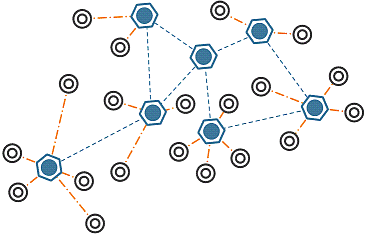
\includegraphics[width=0.5\linewidth]{figures/wsn.png}
  
\end{figure}

\end{frame}
\end{withoutheadline}
%%%%%%%%%%%%%%%%%%%%%%%%%%%%%%%%%%   2   %%%%%%%%%%%%%%%%%%%%%%%%%%%%%%%%

\begin{withoutheadline}
\begin{frame}{General intoduction}{IEEE802.15.4}

\setbeamercolor{block title}{bg=blue!30,fg=black}
\setbeamercolor{block body}{bg=blue!10,fg=black}
\setbeamertemplate{blocks}[rounded][shadow=false]


\begin{minipage}[t]{0.48\linewidth}

\begin{block}{Converge Cast Structure}
    \begin{itemize}
    \item Nodes radio range defines the neighborhood.
    \item<2-> \alert{Sink} is selected. 
    \item<3-> Packets are forwarded \alert{toward the sink}.
    \item<4-> Communication pairs.
    \end{itemize}
    \end{block}
\end{minipage}\hfill
\begin{minipage}[t]{0.48\linewidth}
\centering
 \begin{figure}[p]

 \only<1>{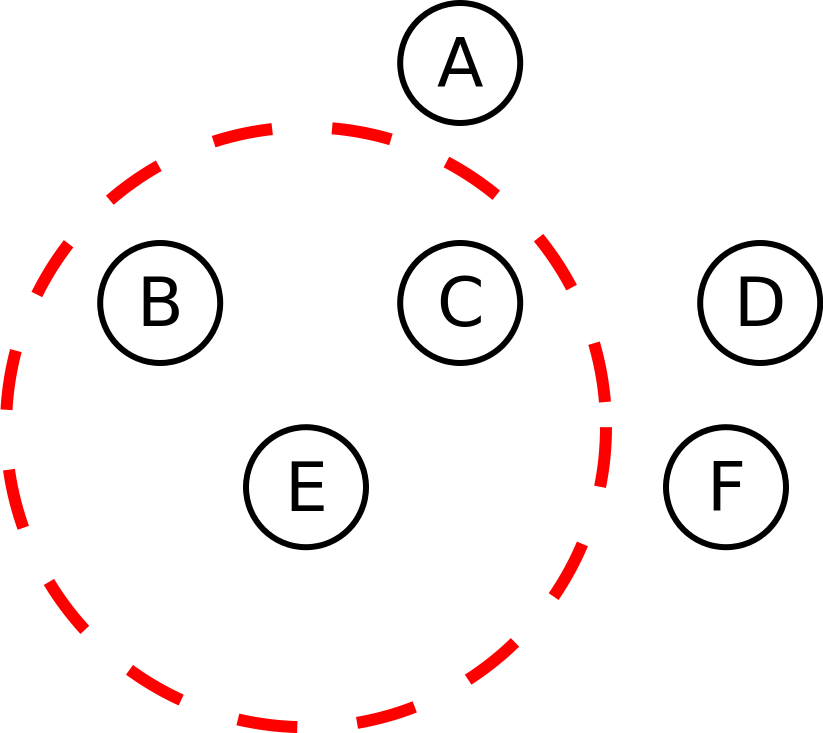
\includegraphics[width=\linewidth]{figures/map1.png}}
  \only<2>{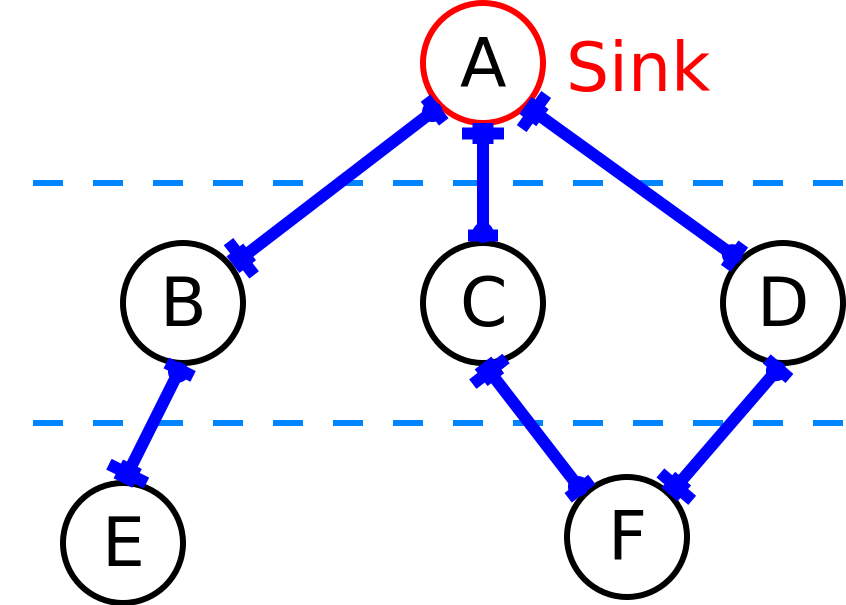
\includegraphics[width=\linewidth]{figures/map2.png}}
  \only<3>{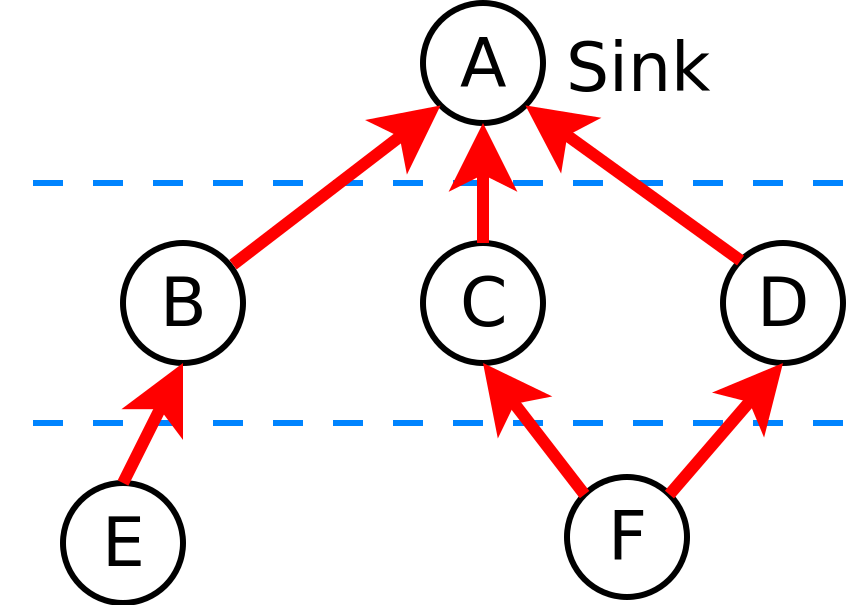
\includegraphics[width=\linewidth]{figures/map3.png}}
  \only<4>{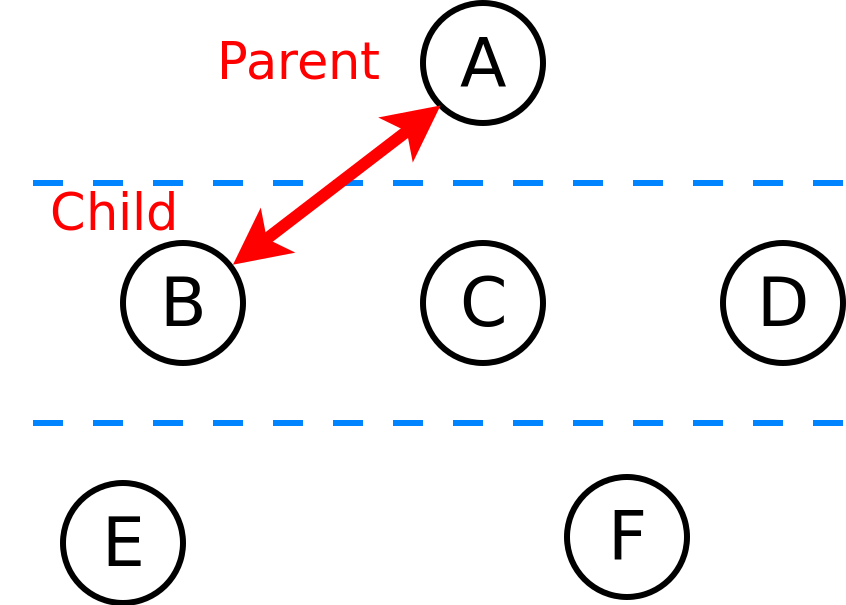
\includegraphics[width=\linewidth]{figures/map4.png}}
  
\end{figure}
\end{minipage}

   
    
    

\end{frame}
\end{withoutheadline}

%%%%%%%%%%%%%%%%%%%%%%%   IEEE802.15.4 Protocols  %%%%%%%%%%%%%%%%%%%%%%%
\subsection{IEEE802.15.4 Protocols}
%%%%%%%%%%%%%%%%%%%%%%%%%%%%%%%%%%   3   %%%%%%%%%%%%%%%%%%%%%%%%%%%%%%%%
\begin{withoutheadline}
\begin{frame}{IEEE802.15.4 Protocols}

\setbeamercolor{block title}{bg=blue!30,fg=black}
\setbeamercolor{block body}{bg=blue!10,fg=black}
\setbeamertemplate{blocks}[rounded][shadow=false]

\begin{block}{IEEE802.15.4e TSCH}
    \begin{itemize}
    \item  IEEE802.15.4 defines the MAC and PHY layers. 
    \item  TSCH is an extension of the MAC layer of IEEE802.15.4.
    \item<2->  Time/Frequency multiplexing of the bandwidth.
    \item<3-> Shared cells/Dedicated cells..
    \item<5-> 6TiSCH operation sublayer 6top will manage the TSCH.
    \end{itemize}
    \end{block}

\begin{figure}[p]

 \only<1>{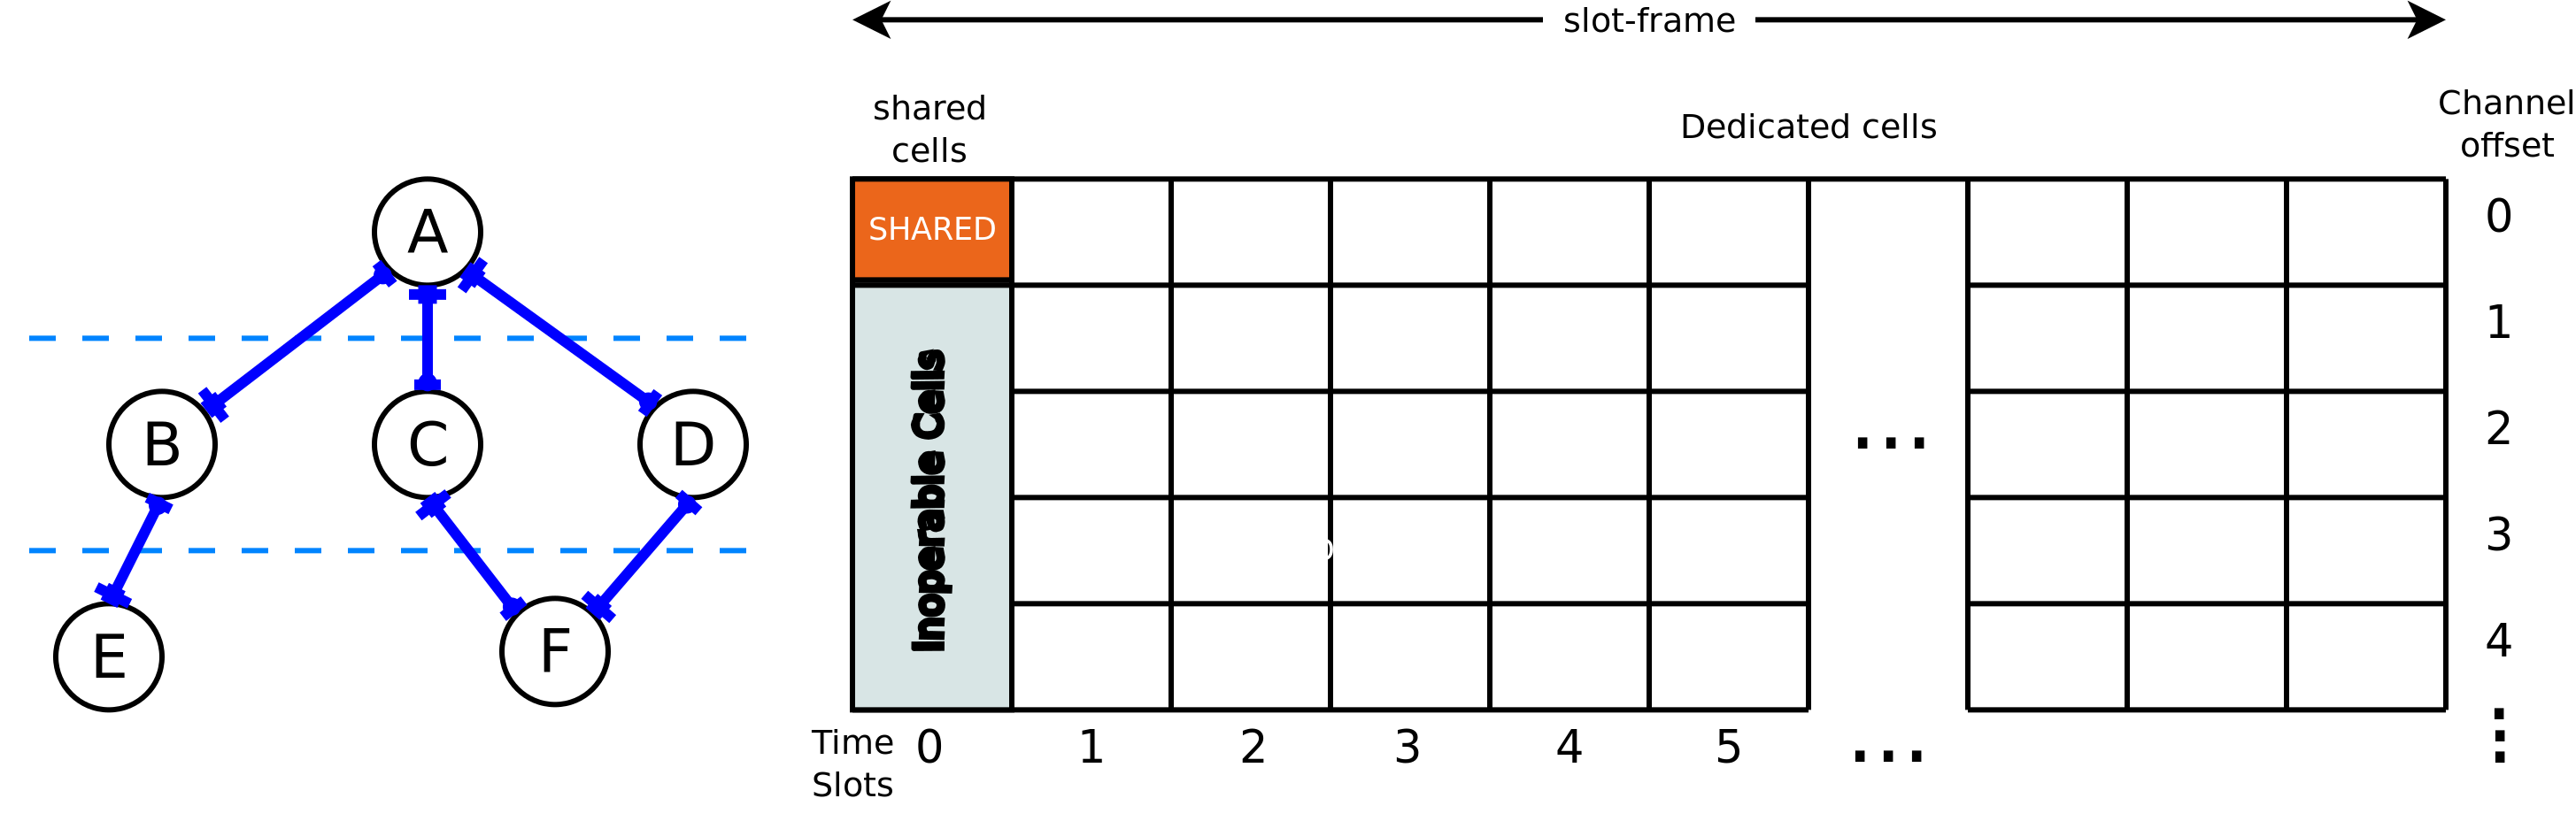
\includegraphics[width=\linewidth]{figures/TSCH1.png}}
  \only<2>{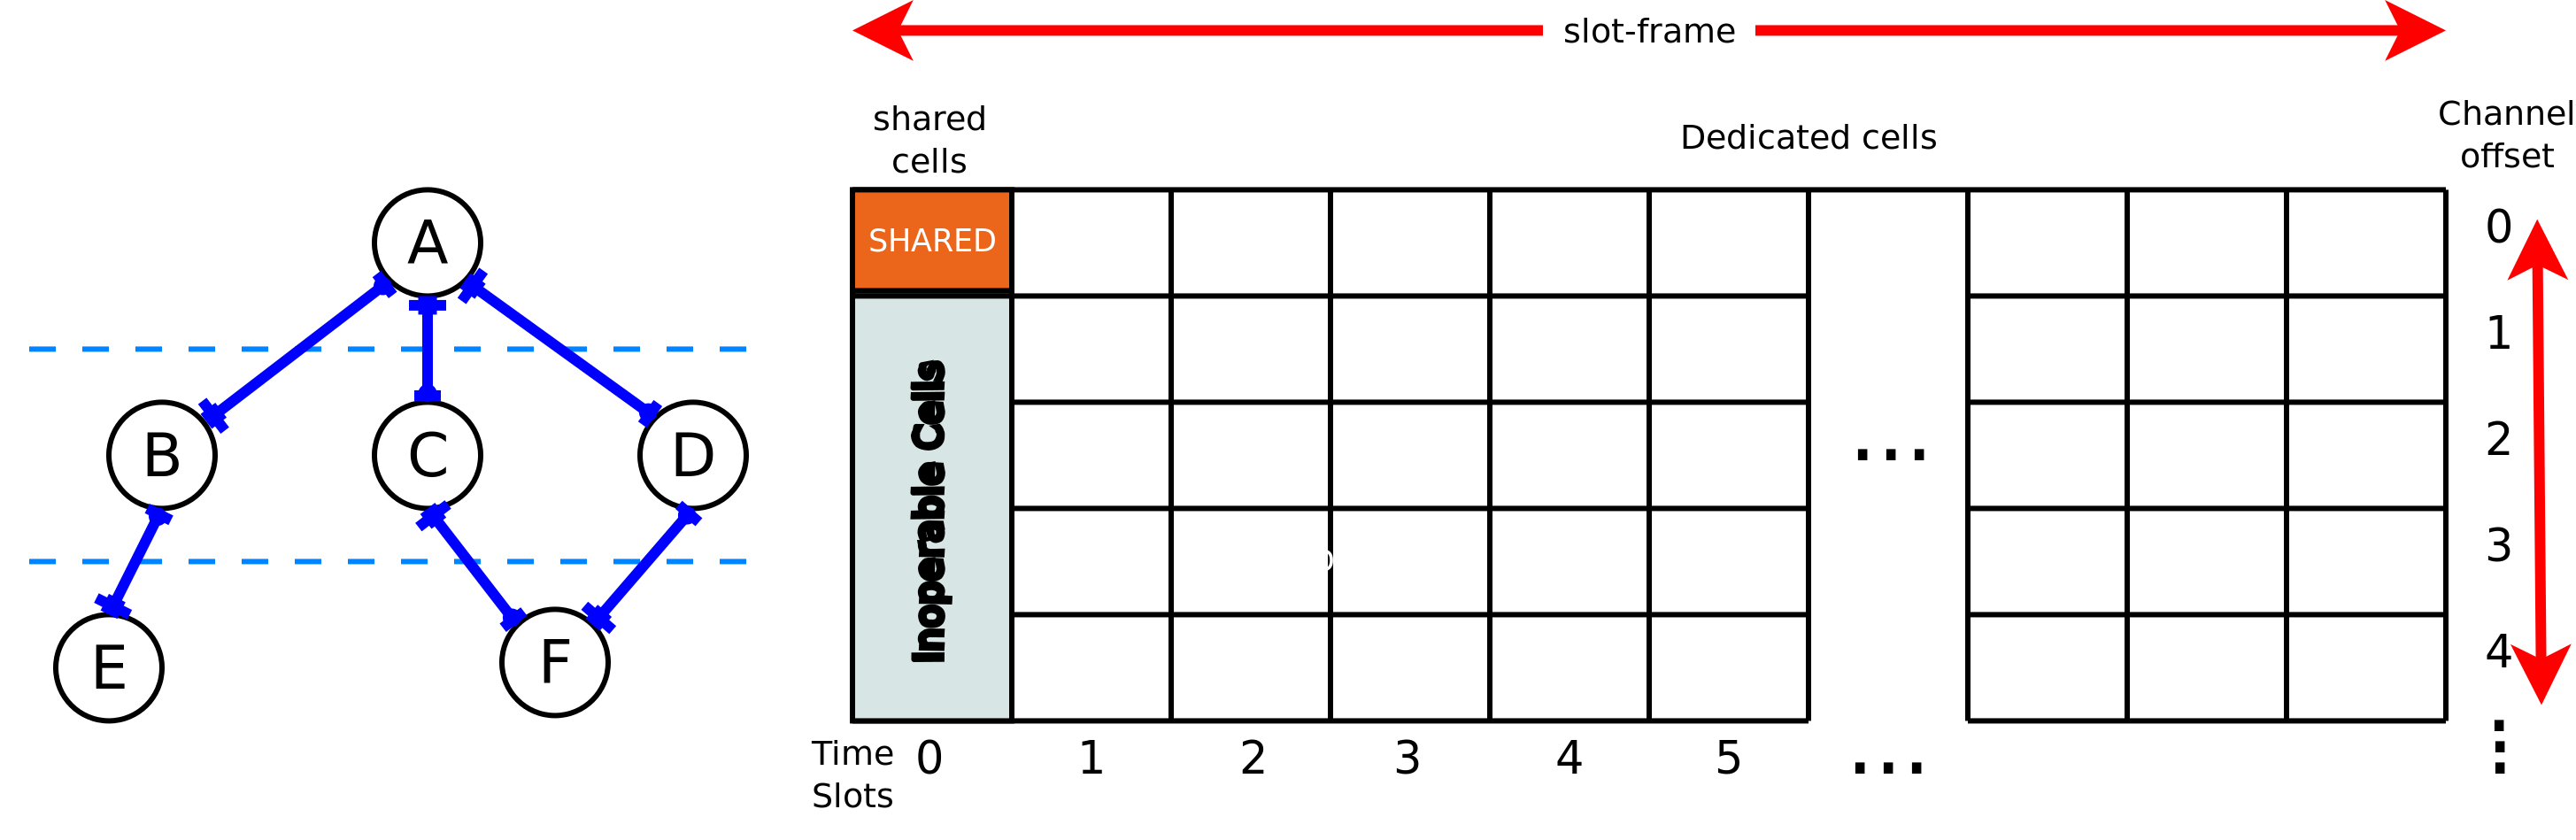
\includegraphics[width=\linewidth]{figures/TSCH2.png}}
  \only<3>{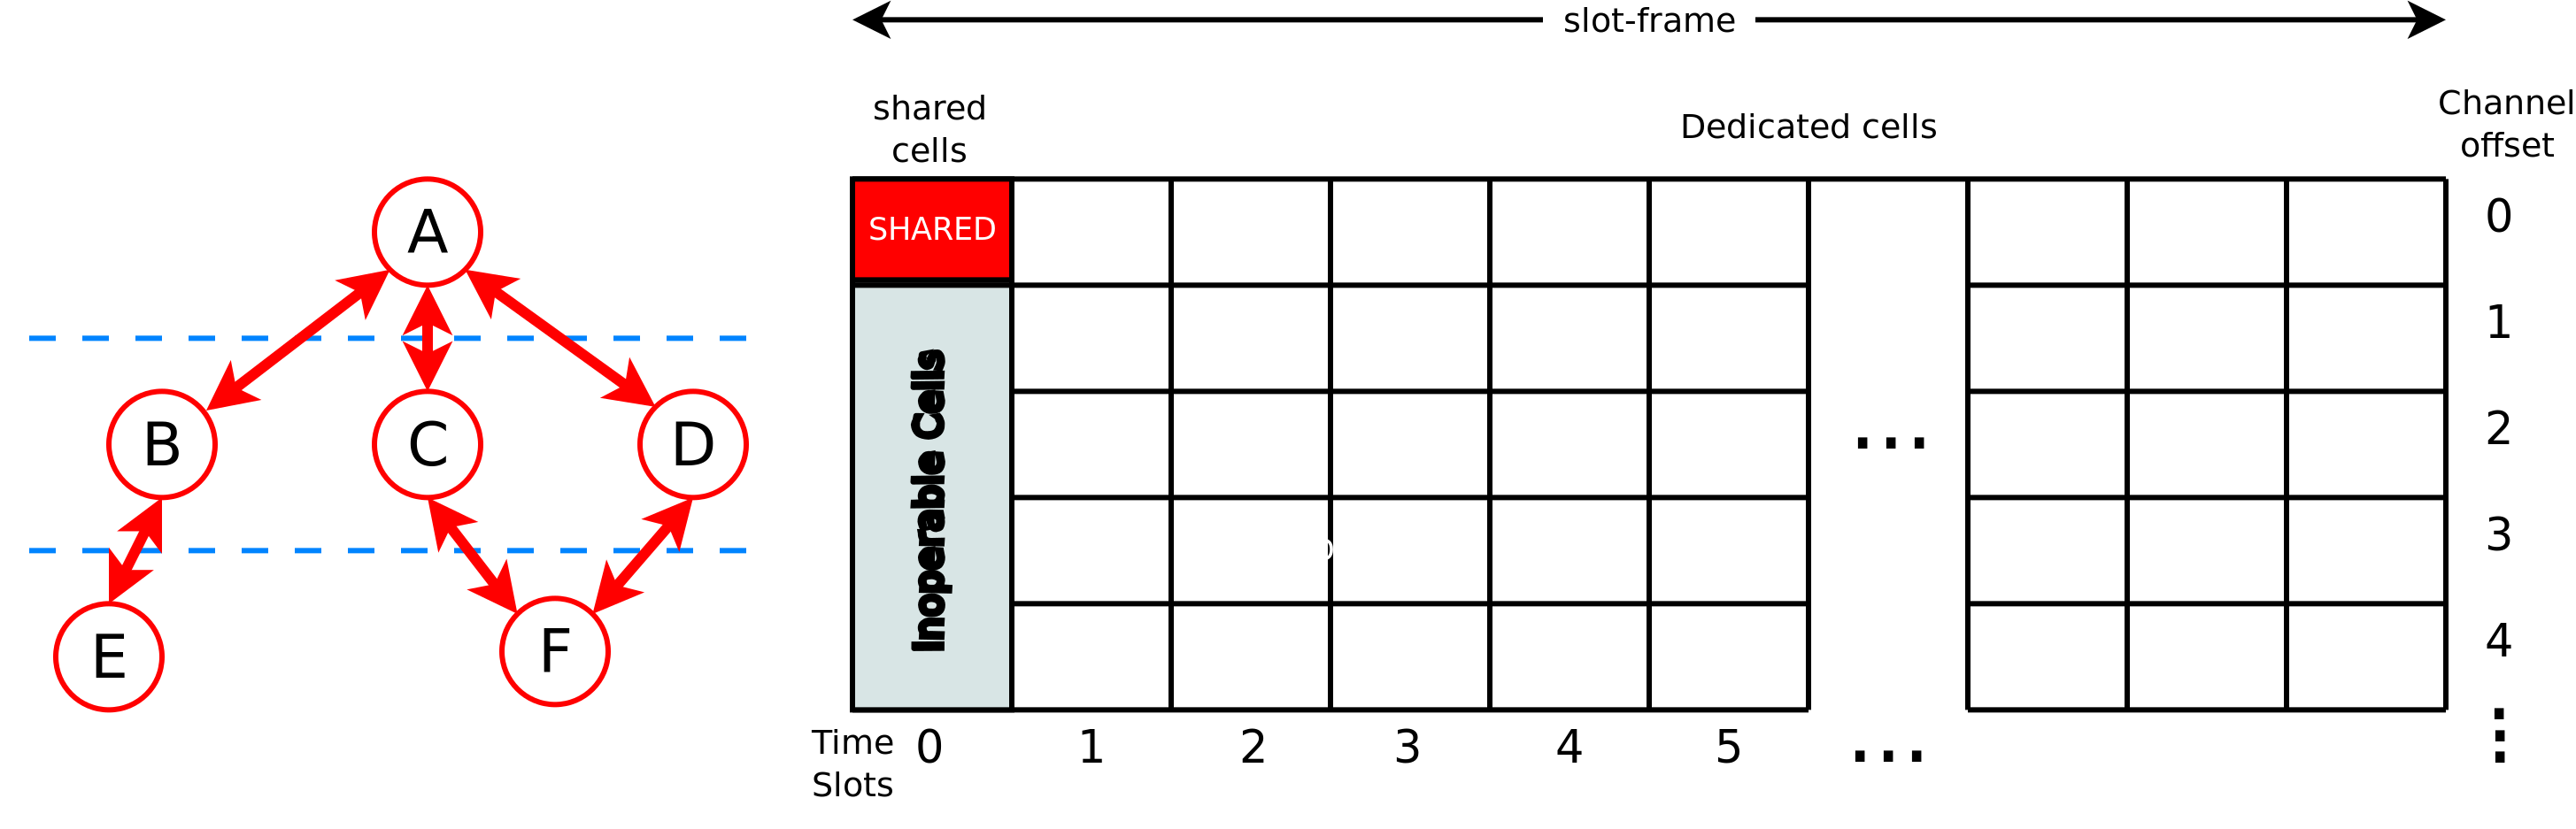
\includegraphics[width=\linewidth]{figures/TSCH3.png}}
      \only<4->{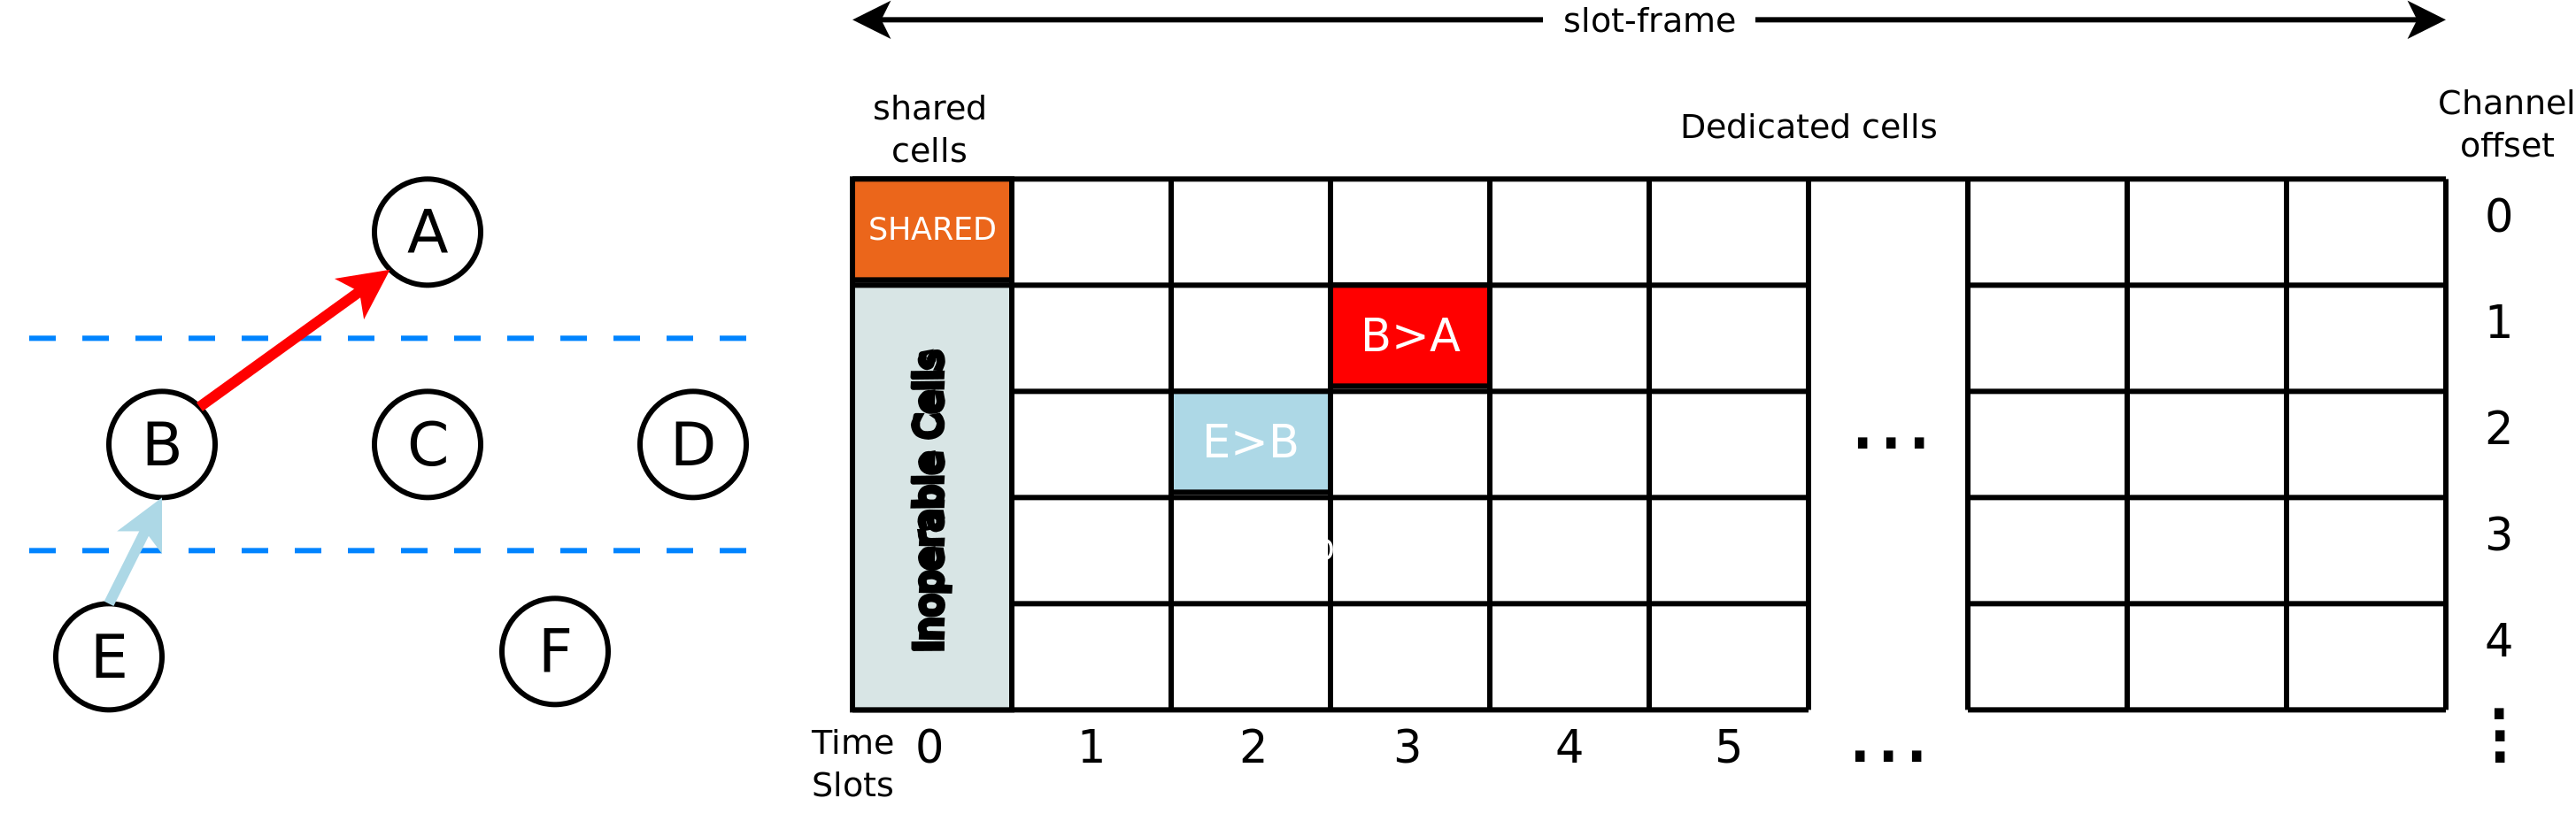
\includegraphics[width=\linewidth]{figures/TSCH5.png}}
\end{figure}


\end{frame}
\end{withoutheadline}
%%%%%%%%%%%%%%%%%%%%%%%%%%%%%%%%%%   4   %%%%%%%%%%%%%%%%%%%%%%%%%%%%%%%%


%%%%%%%%%%%%%%%%%%%%%%%%%%%%%%%%%%  5   %%%%%%%%%%%%%%%%%%%%%%%%%%%%%%%%
\begin{withoutheadline}
\begin{frame}{IEEE802.15.4 Protocols}


\setbeamercolor{block title}{bg=blue!30,fg=black}
\setbeamercolor{block body}{bg=blue!10,fg=black}
\setbeamertemplate{blocks}[rounded][shadow=false]
\begin{block}{Cell Reservation Process}
    \begin{enumerate}
    
    
    \item  Scheduling function decides new cell should be assigned.
    \item<2-> Child node sends an Add request. 
    \item<3-> Scheduling function decides which cells to be selected. 
    \item<4-> Parent node replies with an Add response.
    \item<5-> Cell is added and communication start.
    \end{enumerate}
    \end{block}

\begin{figure}[p]

 \only<1>{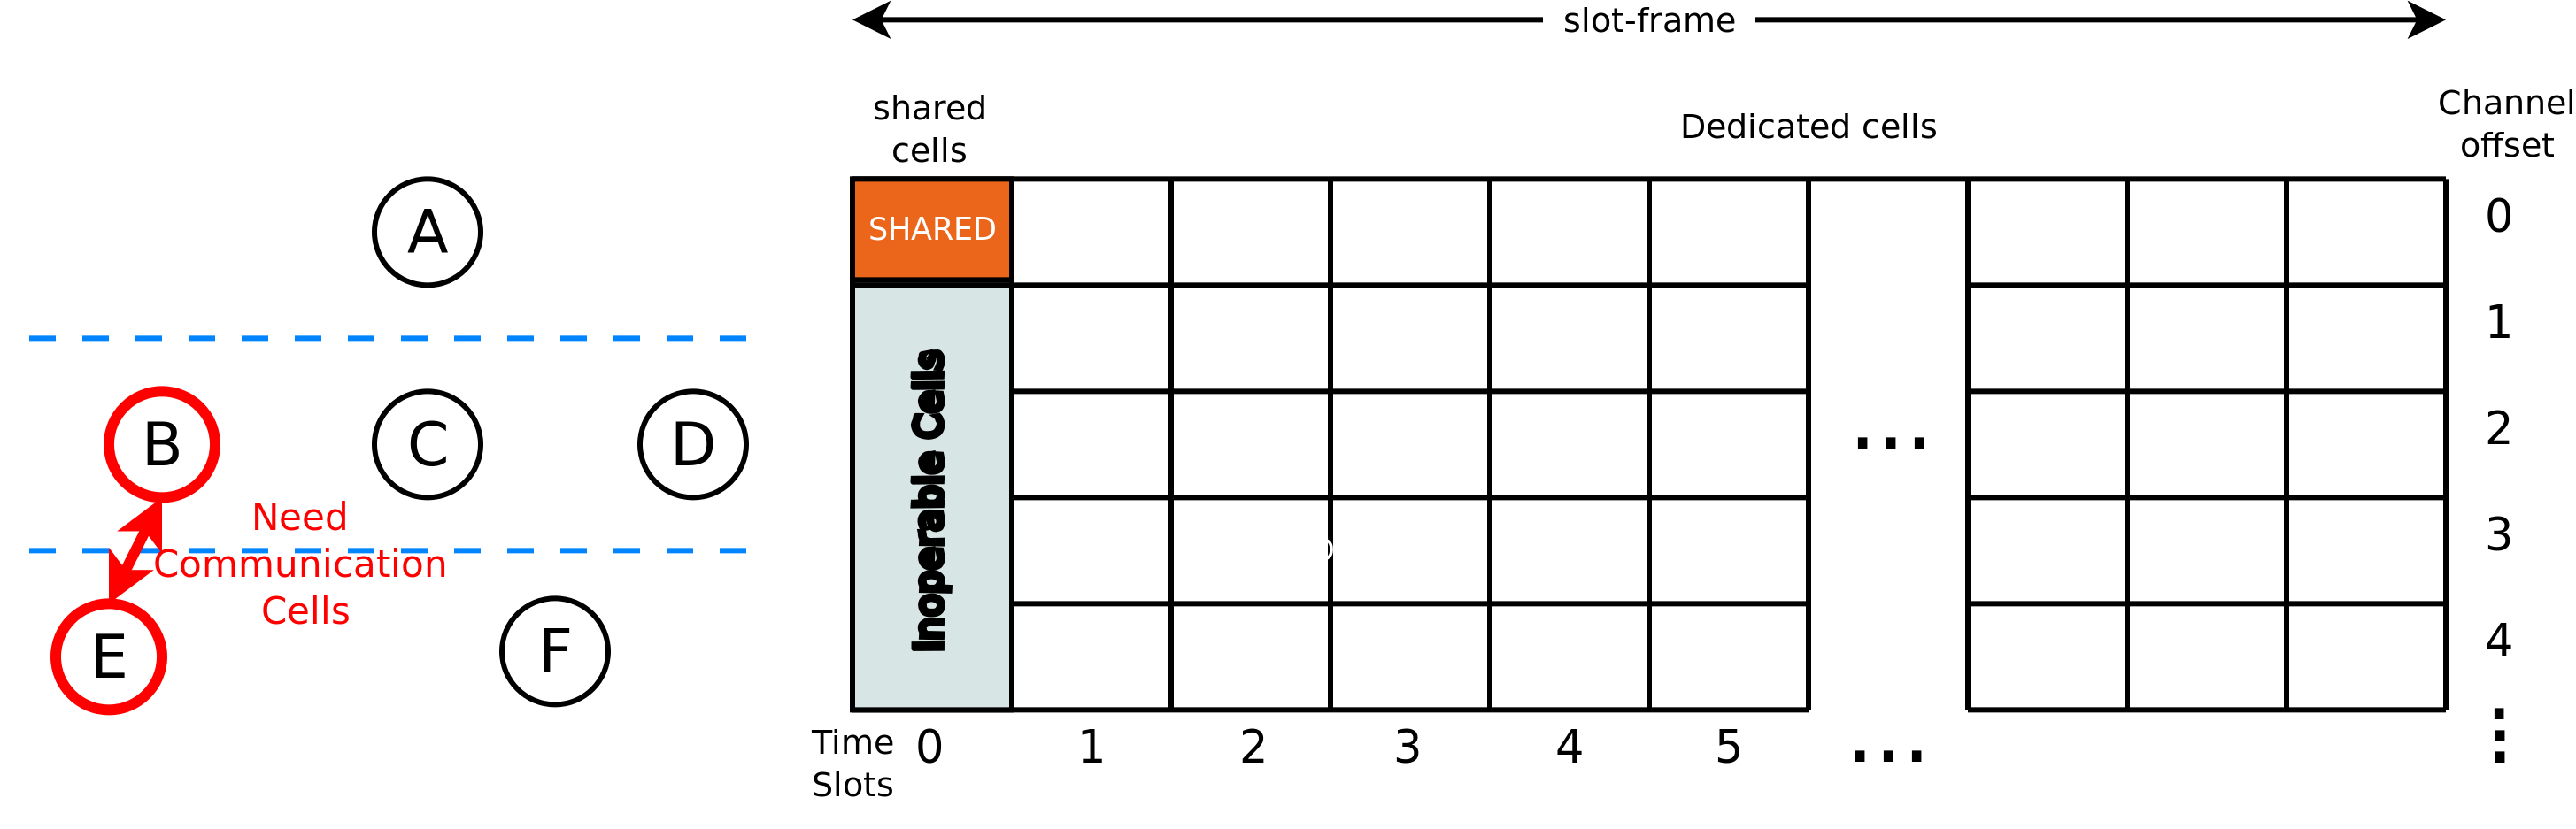
\includegraphics[width=\linewidth]{figures/6top1.png}}
  \only<2>{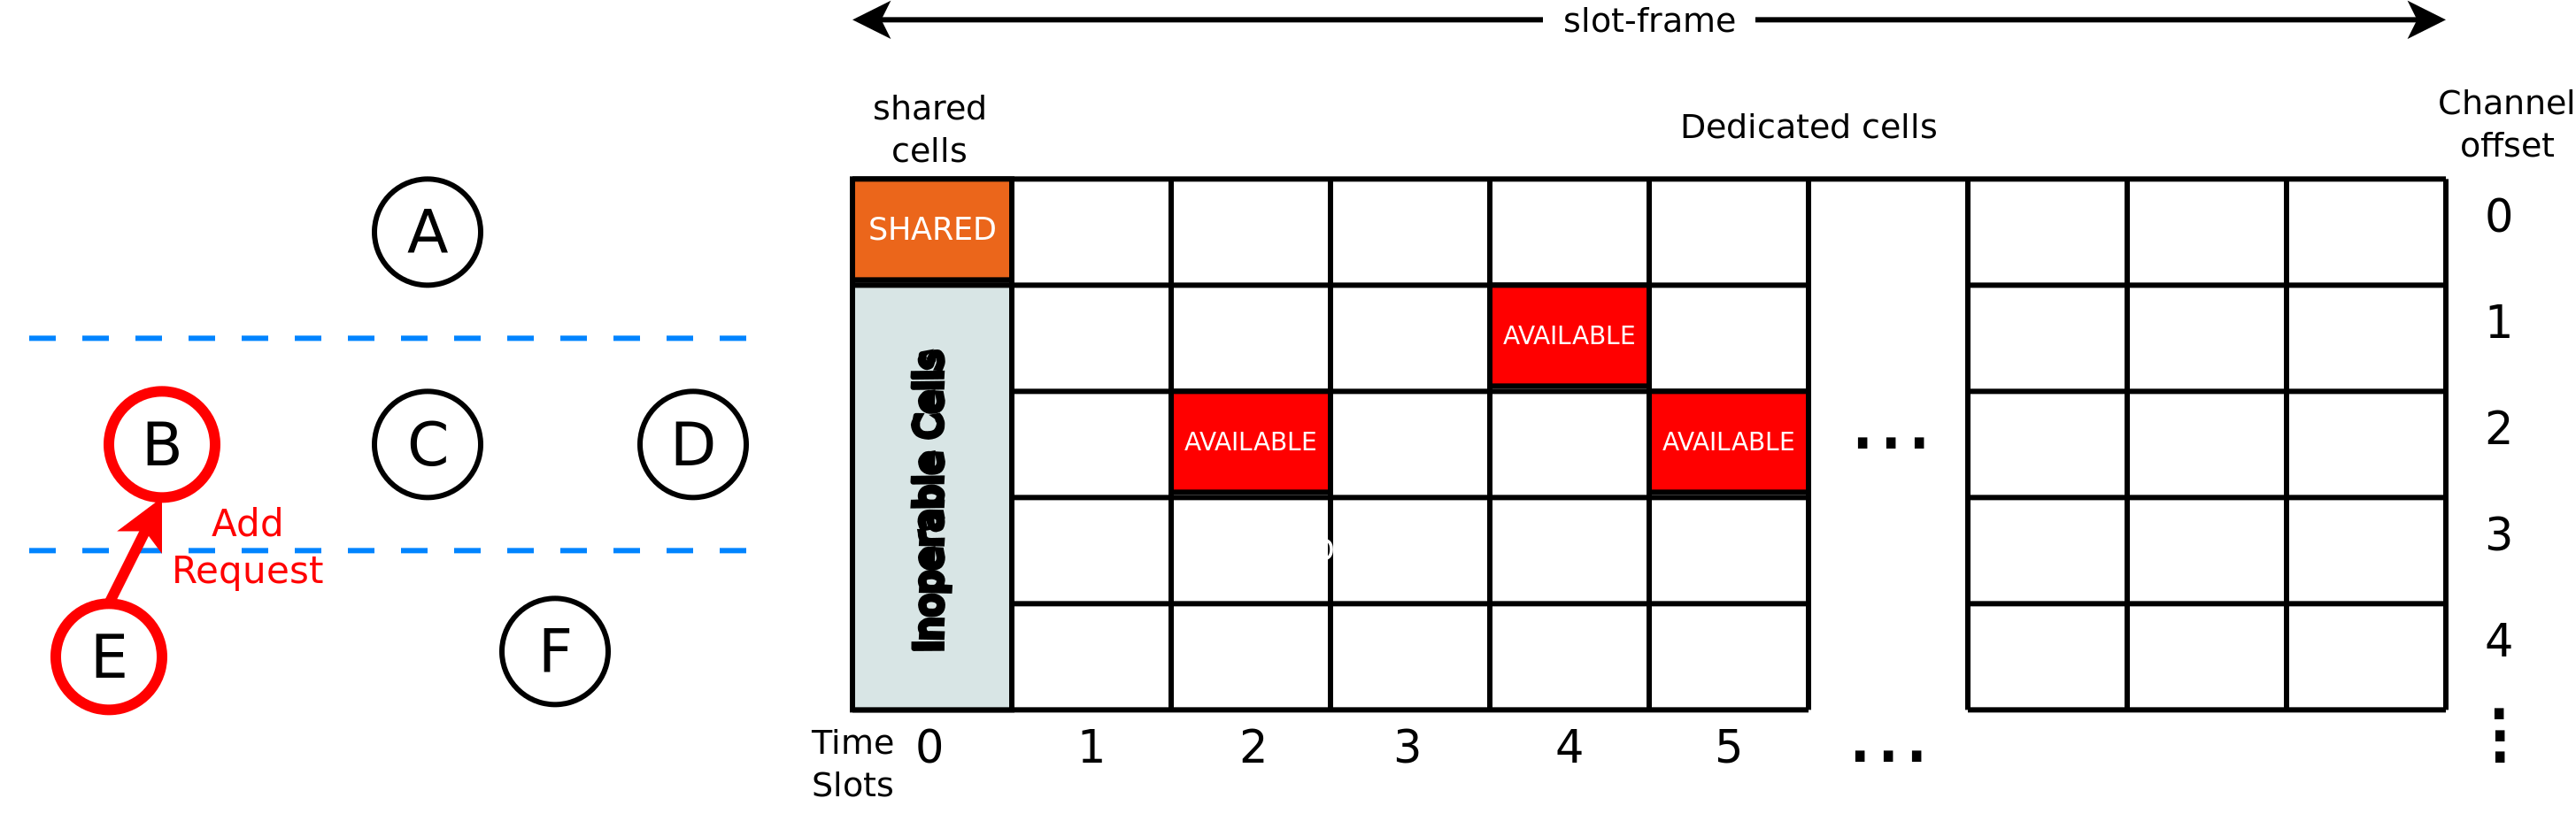
\includegraphics[width=\linewidth]{figures/6top2.png}}
  \only<3>{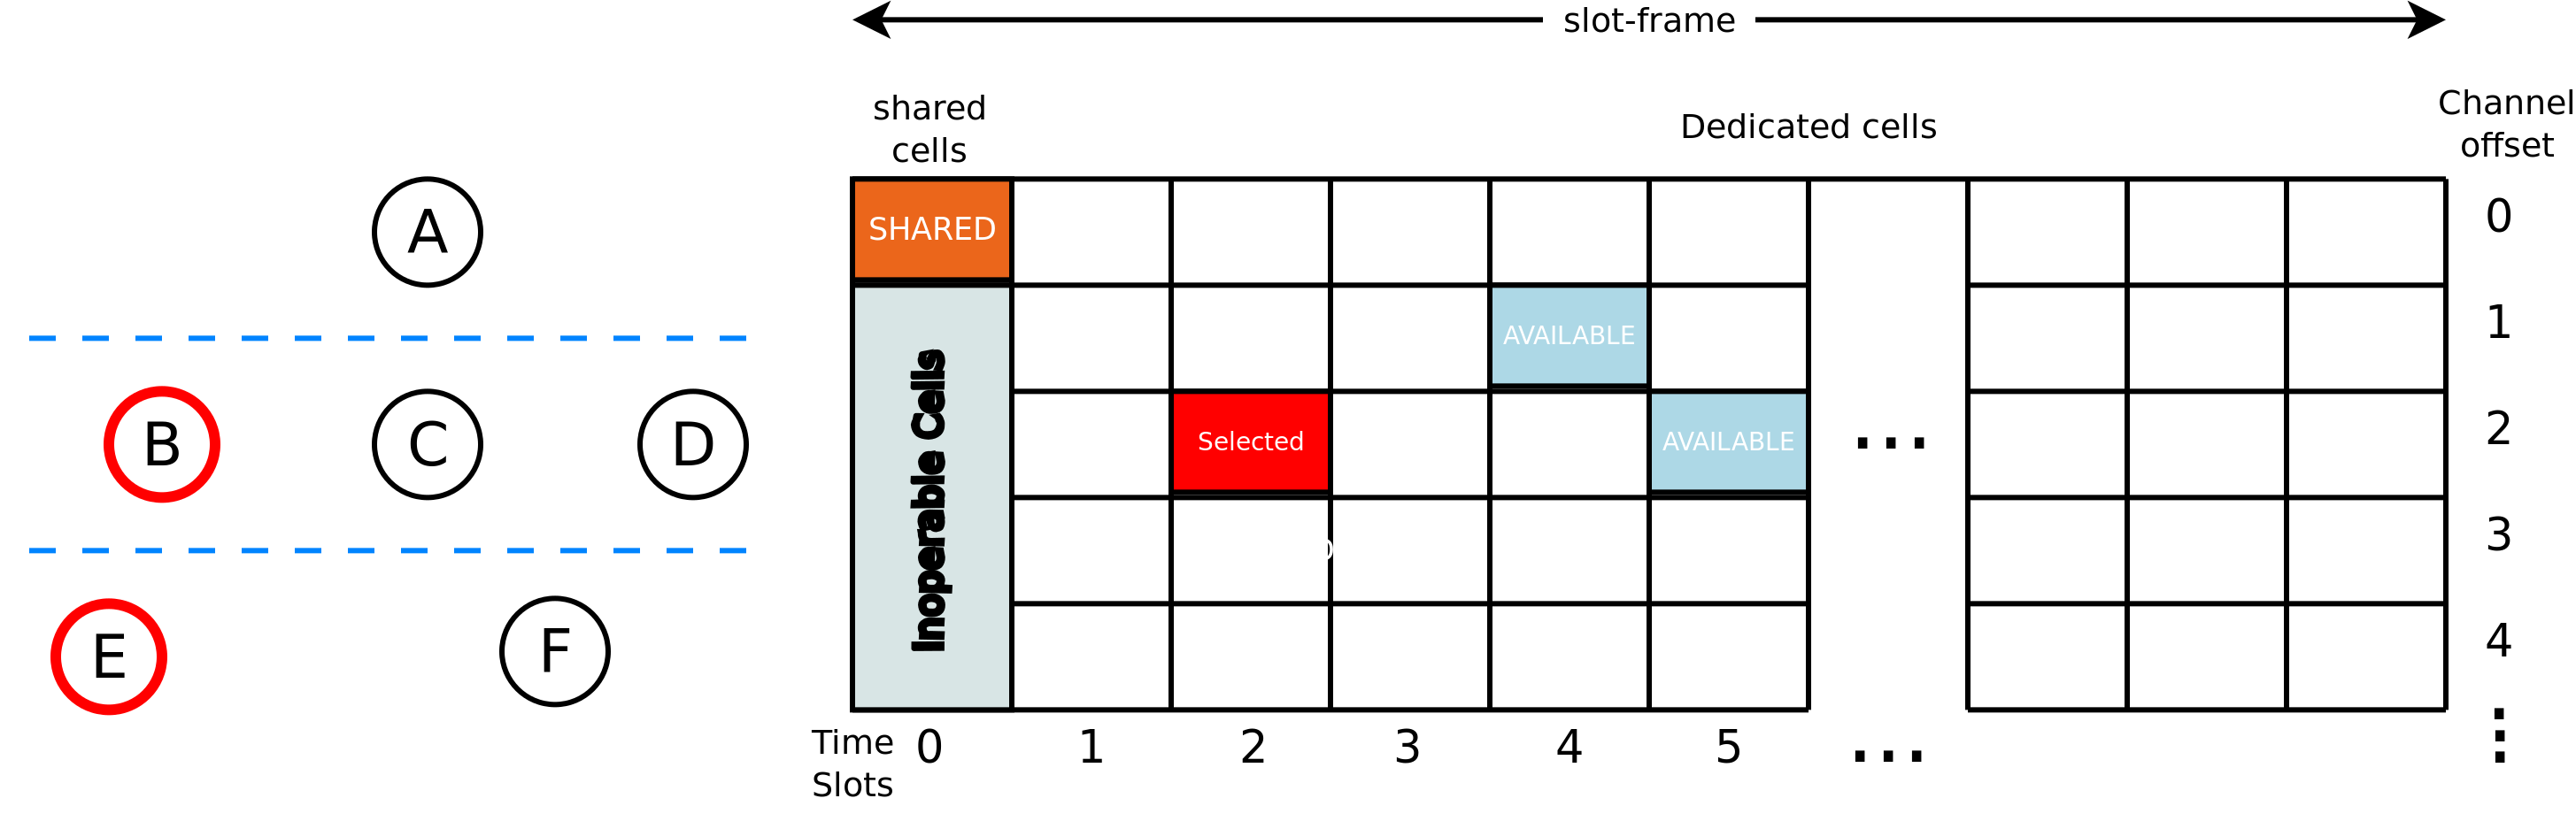
\includegraphics[width=\linewidth]{figures/6top3.png}}
  \only<4>{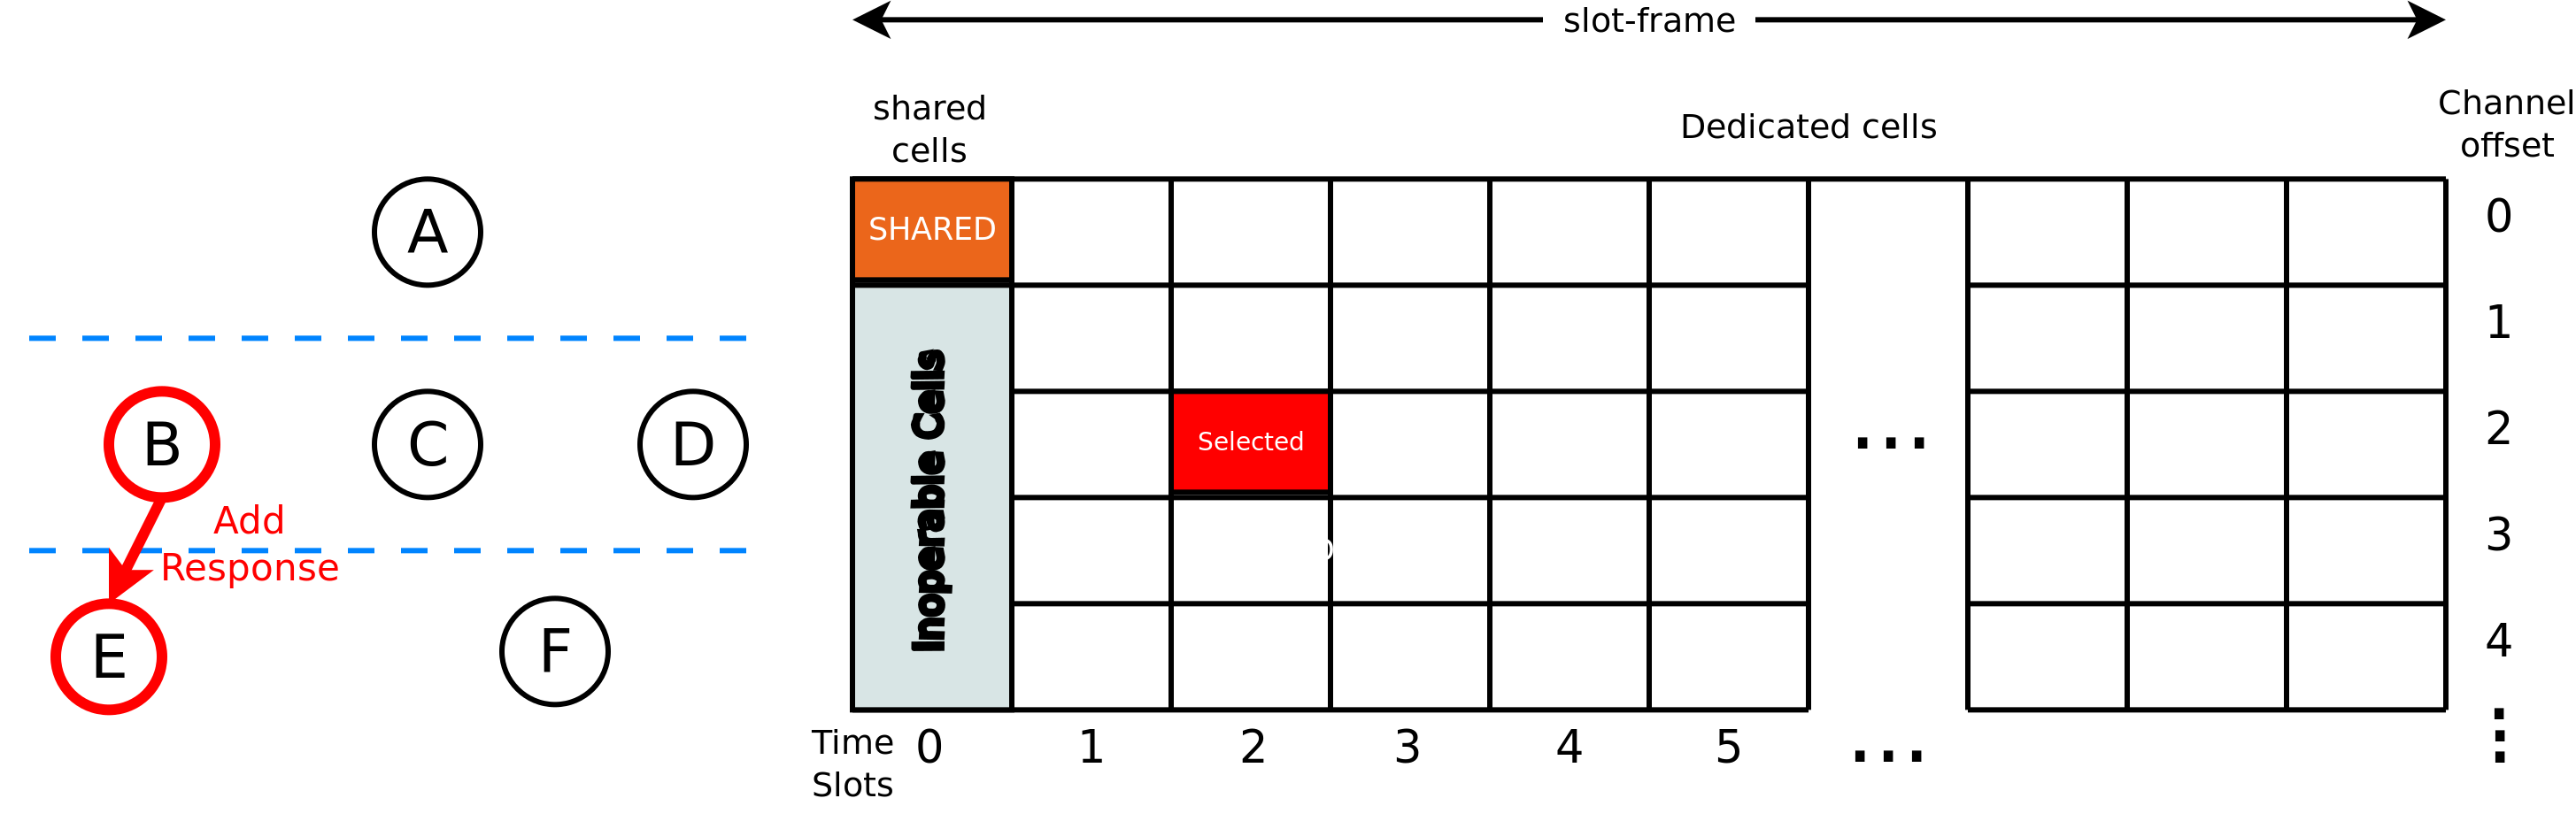
\includegraphics[width=\linewidth]{figures/6top4.png}}
    \only<5>{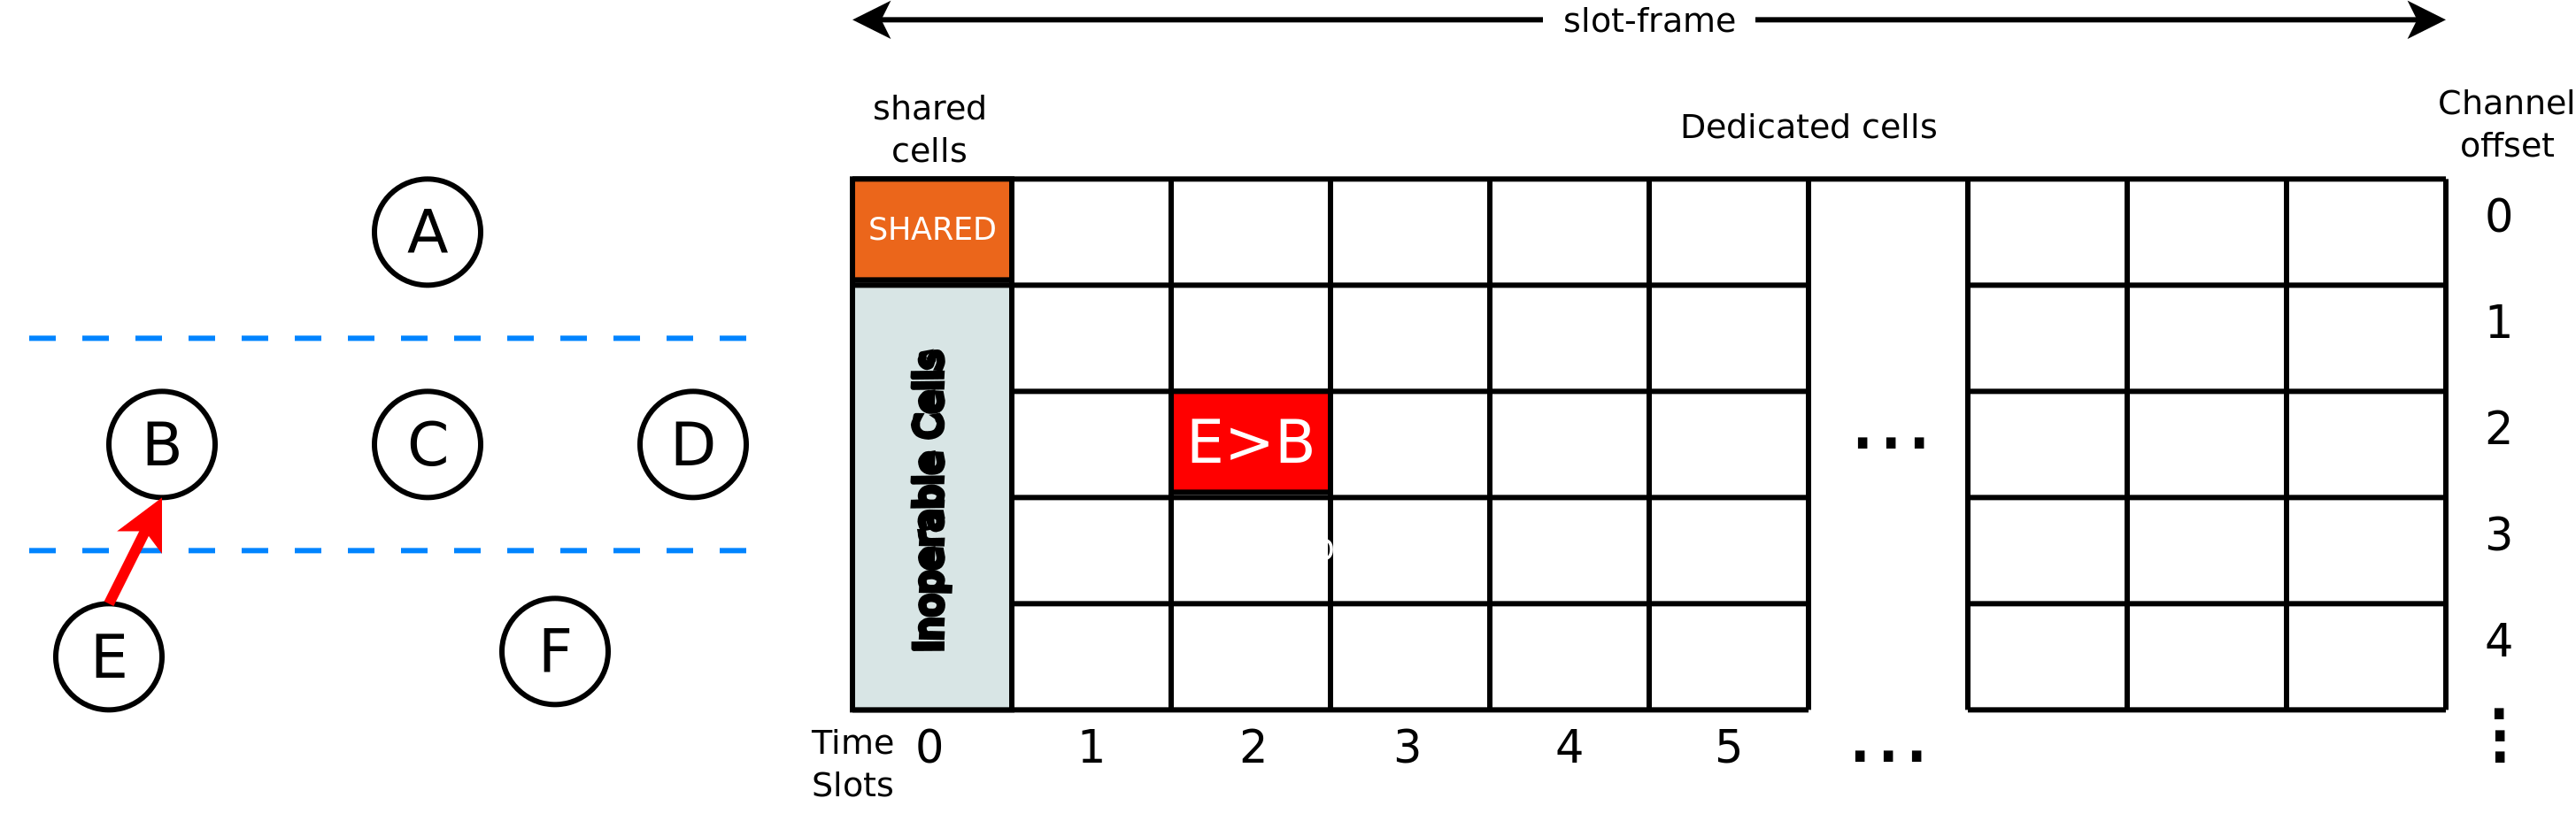
\includegraphics[width=\linewidth]{figures/6top5.png}}
\end{figure}




\end{frame}
\end{withoutheadline}

%%%%%%%%%%%%%%%%%%%%%%%%%%%%%%  Objectives  %%%%%%%%%%%%%%%%%%%%%%%%%%%%

\subsection{Project challenges \& Objectives}
%%%%%%%%%%%%%%%%%%%%%%%%%%%%%%%%%%  6   %%%%%%%%%%%%%%%%%%%%%%%%%%%%%%%%
\begin{withoutheadline}
\begin{frame}{Project challenges \& Objectives}


\setbeamercolor{block title}{bg=blue!30,fg=black}
\setbeamercolor{block body}{bg=blue!10,fg=black}
\setbeamertemplate{blocks}[rounded][shadow=false]

\begin{block}{Collision in Dedicated Cells}
    \begin{itemize}
    \item Collision free Dedicated Cells?  
    \item Neighbor nodes can select the same communication cell.
    \item<3-> Collision at the reception Node.
    
    \end{itemize}
    \end{block}

\begin{figure}[p]

 \only<1>{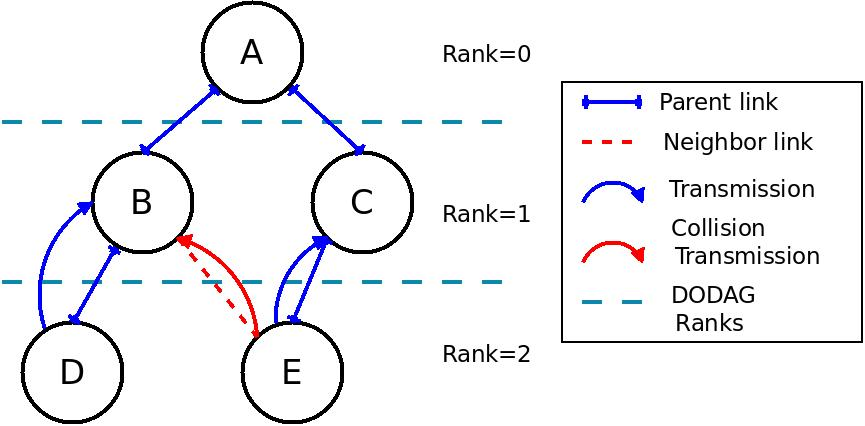
\includegraphics[width=\linewidth]{figures/col1.png}}
  \only<2>{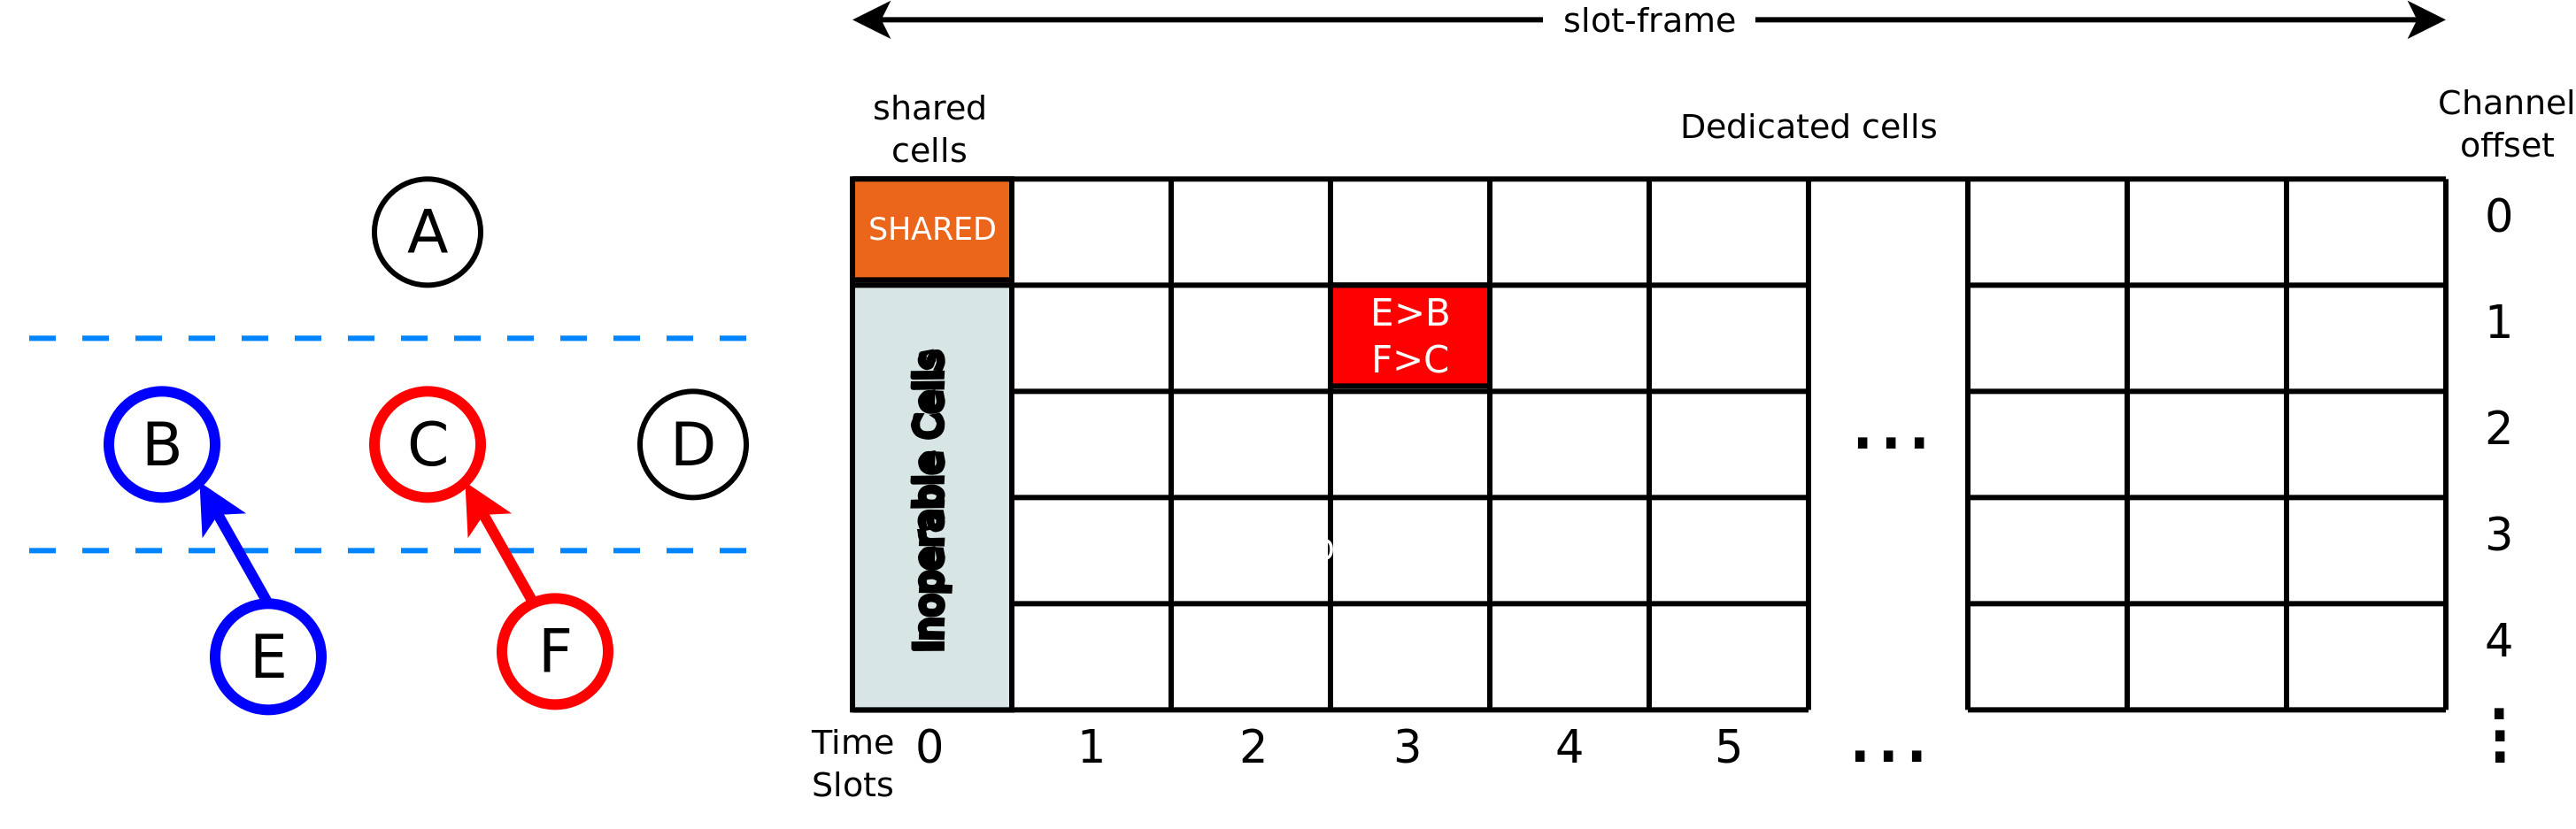
\includegraphics[width=\linewidth]{figures/col2.png}}
  \only<3->{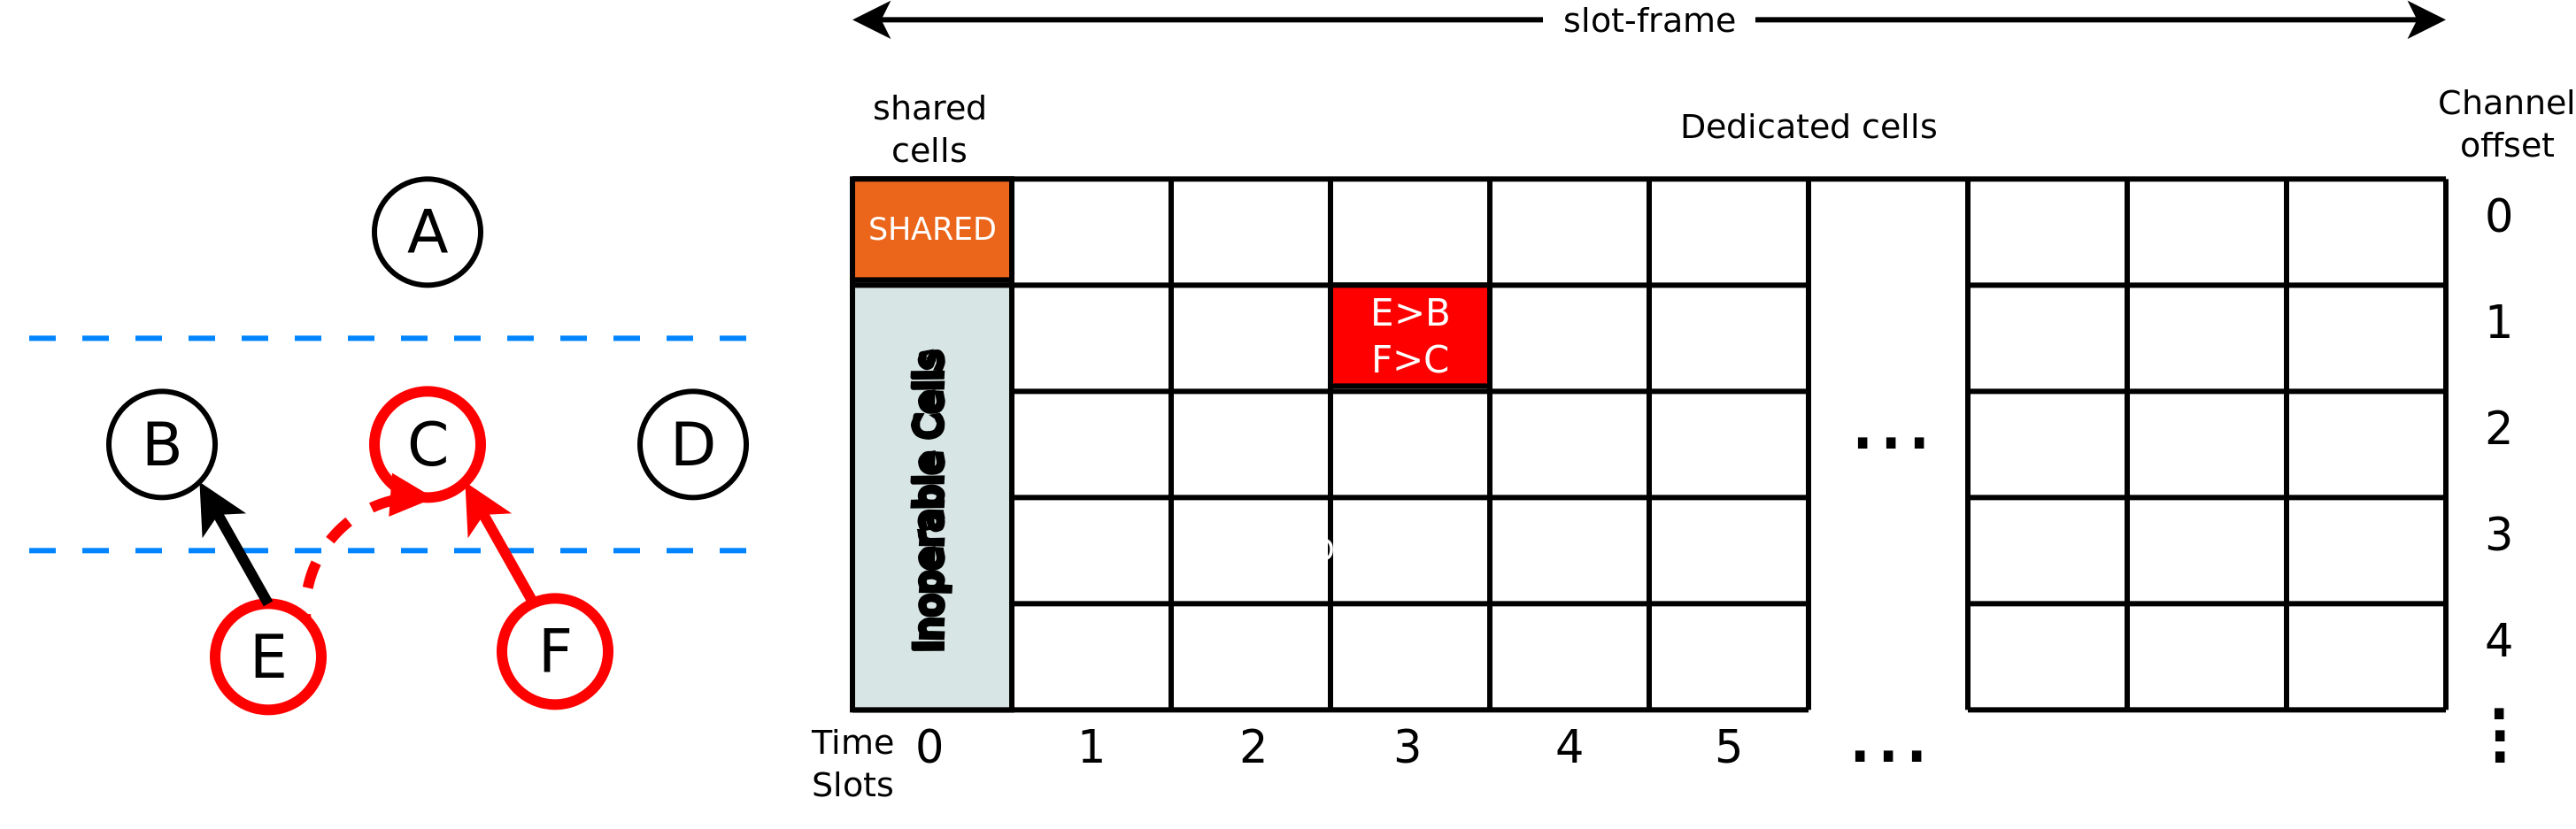
\includegraphics[width=\linewidth]{figures/col3.png}}
  
\end{figure}


\end{frame}
\end{withoutheadline}

%%%%%%%%%%%%%%%%%%%%%%%%%%%%%%%%%%  7   %%%%%%%%%%%%%%%%%%%%%%%%%%%%%%%%



%%%%%%%%%%%%%%%%%%%%%%%%%%%%%%%%%%  8   %%%%%%%%%%%%%%%%%%%%%%%%%%%%%

\begin{withoutheadline}
\begin{frame}{Project Objectives}
\begin{itemize}
\item {Reducing the collisions in TSCH dedicated cells.}
  \item<2-> {Modifying the Cell reserving process without introducing new overhead on the network}
  \item<3-> {Creating a flexible mechanism, compatible with all scheduling functions }

\end{itemize}

\end{frame}
\end{withoutheadline}

\section{Proposed Mechanism}

\subsection{Using 6top Transaction}
\addtocounter{framenumber}{-1}
\begin{withoutheadline}
\begin{frame}{Using 6top Transaction}


\setbeamercolor{block title}{bg=blue!30,fg=black}
\setbeamercolor{block body}{bg=blue!10,fg=black}
\setbeamertemplate{blocks}[rounded][shadow=false]

\begin{block}{Why?}
    \begin{itemize}
    \item  Submitted in the shared slot.
    \item Contains the reserved cells.
    \end{itemize}
    \end{block}


\begin{block}{How?}
    \begin{itemize}
    \item The child node Sends an Add Request.
    \item<2-> The parent replies with the selected cells.
    \item<3-> The neighboring nodes collects the reserved cells and save them. 
    \end{itemize}
    \end{block}
    
    
\begin{figure}[p]

 
  \only<1>{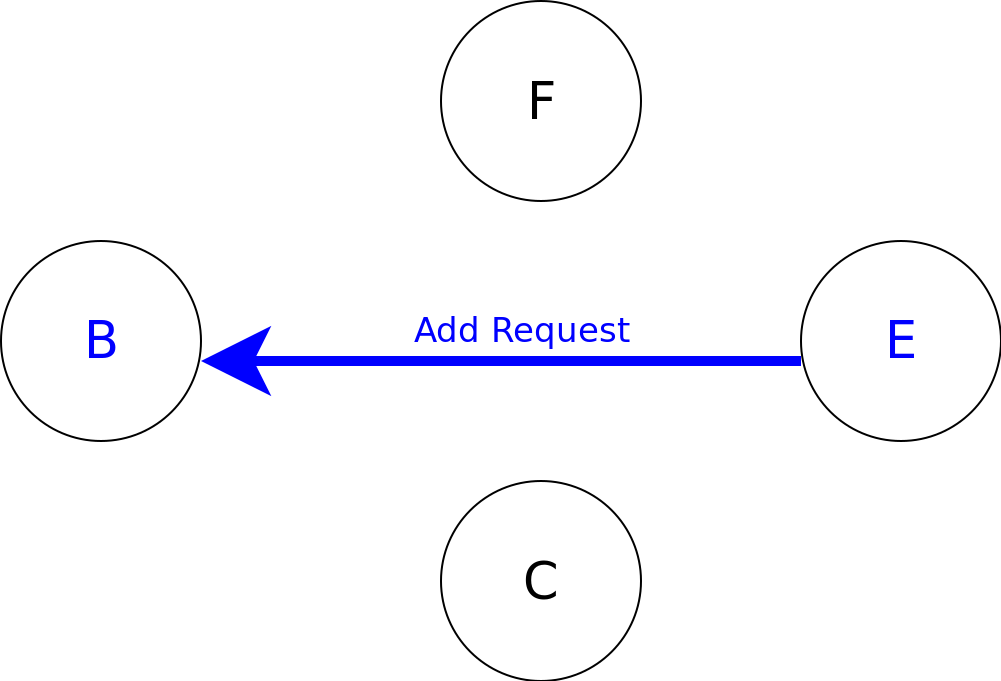
\includegraphics[width=.4\linewidth]{figures/usin1.png}}
  \only<2>{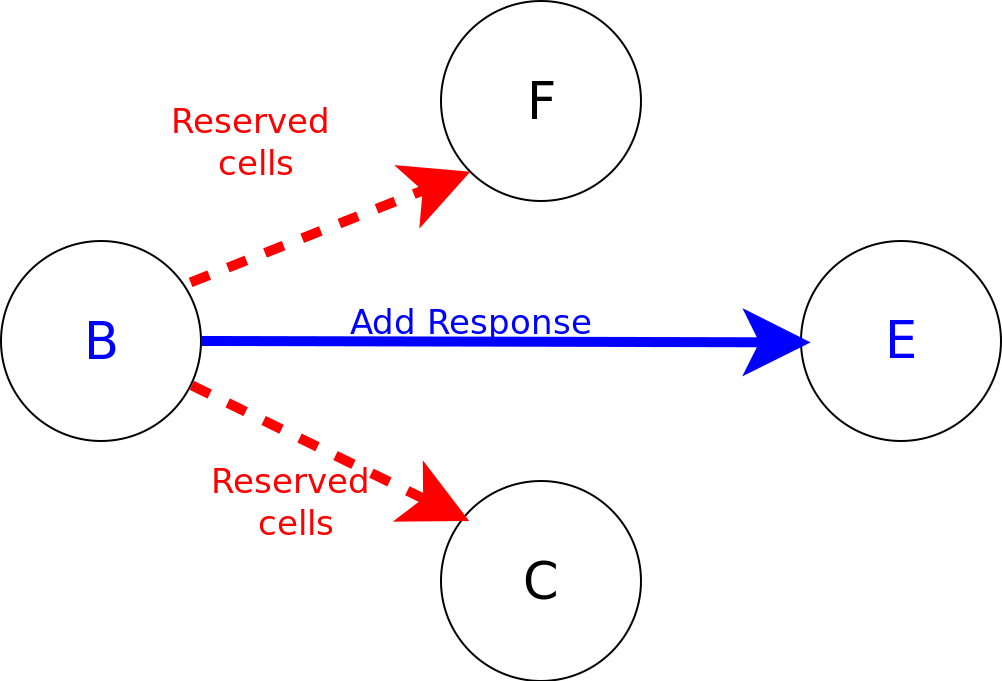
\includegraphics[width=.4\linewidth]{figures/usin2.png}}
  \only<3>{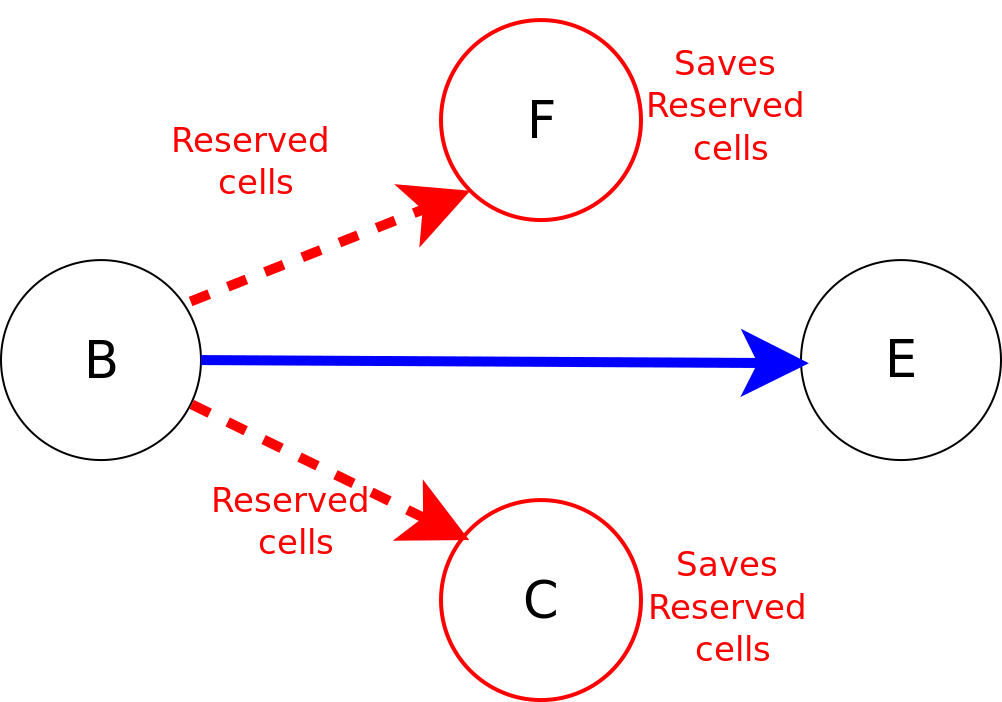
\includegraphics[width=.4\linewidth]{figures/usin3.png}}
\end{figure}

\end{frame}
\end{withoutheadline}

\subsection{Avoid Table}


\addtocounter{framenumber}{-1}
\begin{withoutheadline}
\begin{frame}{Avoid Table structure and functioning}


\setbeamercolor{block title}{bg=blue!30,fg=black}
\setbeamercolor{block body}{bg=blue!10,fg=black}
\setbeamertemplate{blocks}[rounded][shadow=false]
\begin{block}{Avoid Table}
    \begin{itemize}
     \item The cells reserved by neighbors will be saved by a structure similar to that of TSCH table. 
    \item<2-> Scheduling function will avoid selecting cells found in this structure. 
    \item<3-> 6top will manage this table.
    \end{itemize}
    \end{block}
    
    
\begin{figure}[p]

 
  \only<1>{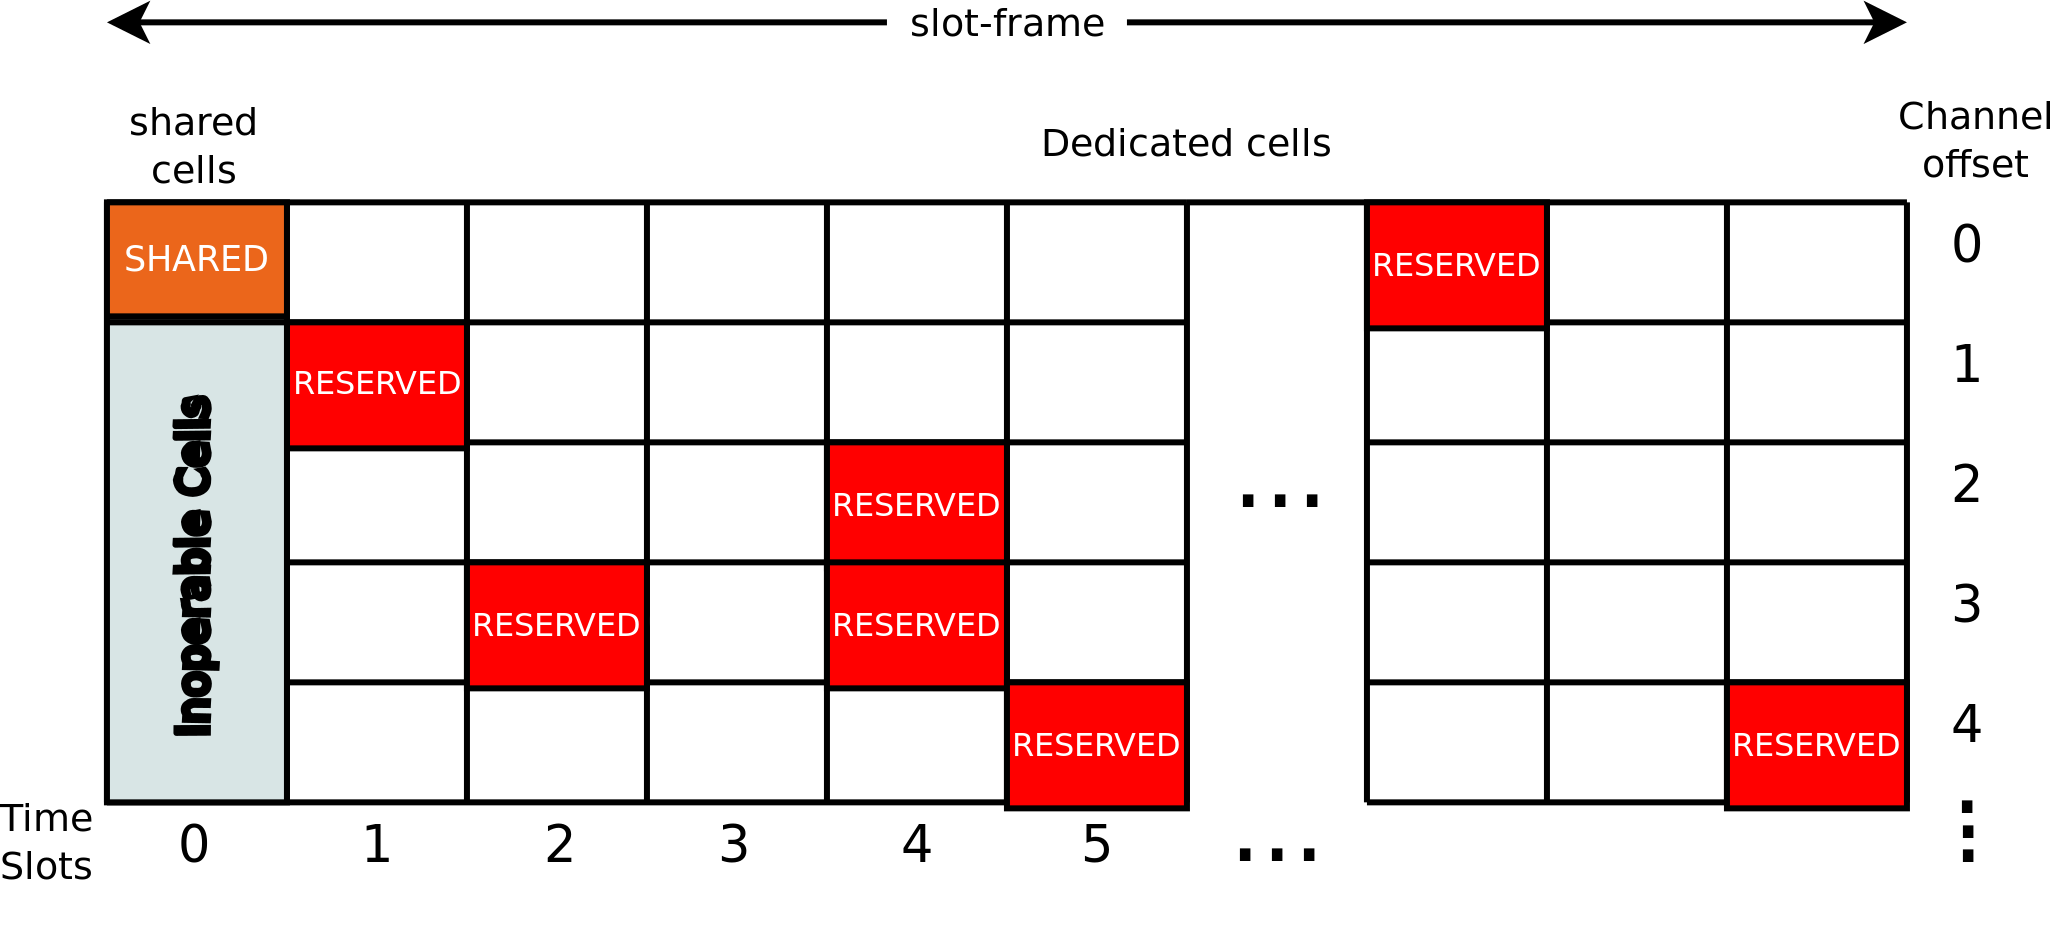
\includegraphics[width=.8\linewidth]{figures/avoid.png}}
  \only<2->{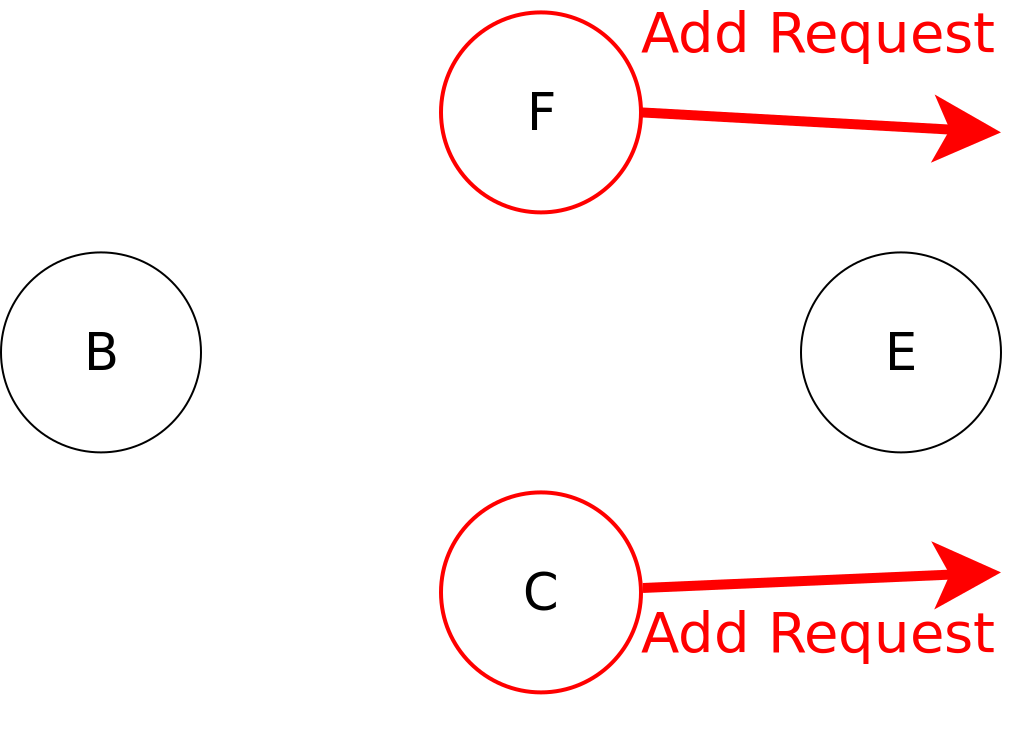
\includegraphics[width=.4\linewidth]{figures/avoid2.png}}
 
\end{figure}



\end{frame}
\end{withoutheadline}


\subsection{Cell Buffer}
\addtocounter{framenumber}{-1}
%% edit 
\begin{withoutheadline}
\begin{frame}{Cell Buffer}
\setbeamercolor{block title}{bg=blue!30,fg=black}
\setbeamercolor{block body}{bg=blue!10,fg=black}
\setbeamertemplate{blocks}[rounded][shadow=false]

\begin{block}{Why?}
\begin{itemize}

\item Some of the 6top Transaction are lost. 
\item Number of the neighbors will not receive the reserved cells. 

\end{itemize}
\end{block}

\begin{block}{How?}
\begin{itemize}


\item Creating a cell buffer that will contain k reserved cells for each node. 
\item<2-> Transmitting the cell buffer each time a cell is reserved.
\end{itemize}
\end{block}
\centering
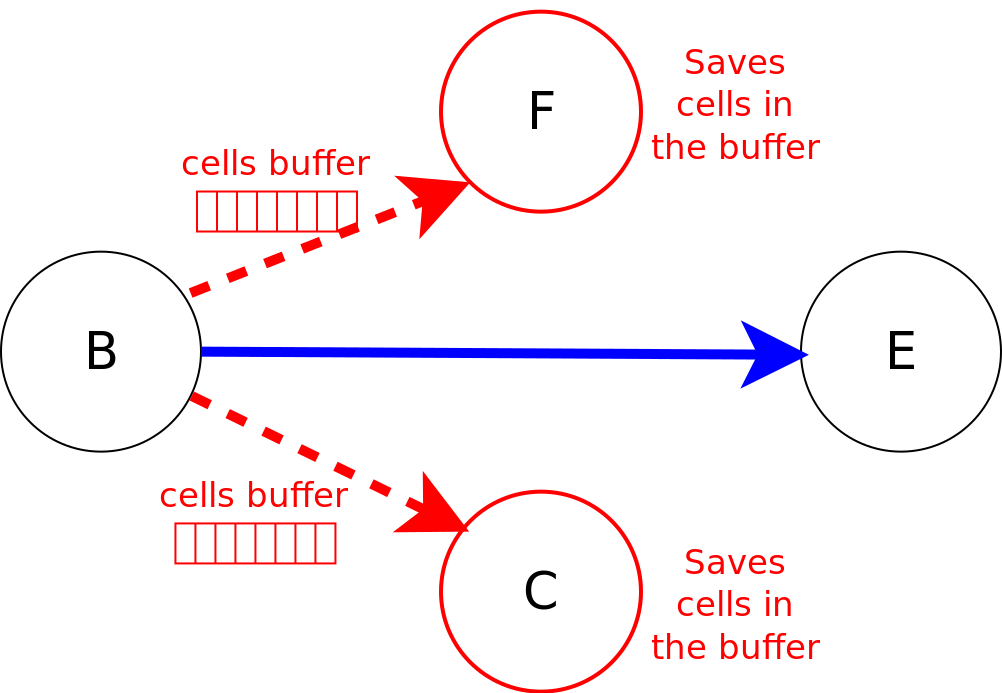
\includegraphics[width=.4\linewidth]{figures/buff.png}

\end{frame}
\end{withoutheadline}
\section{Simulator and Results}
\subsection{Simulator}
\addtocounter{framenumber}{-1}
\begin{withoutheadline}
\begin{frame}{Simulator Architecture}


\setbeamercolor{block title}{bg=blue!30,fg=black}
\setbeamercolor{block body}{bg=blue!10,fg=black}
\setbeamertemplate{blocks}[rounded][shadow=false]

\begin{figure}[p]

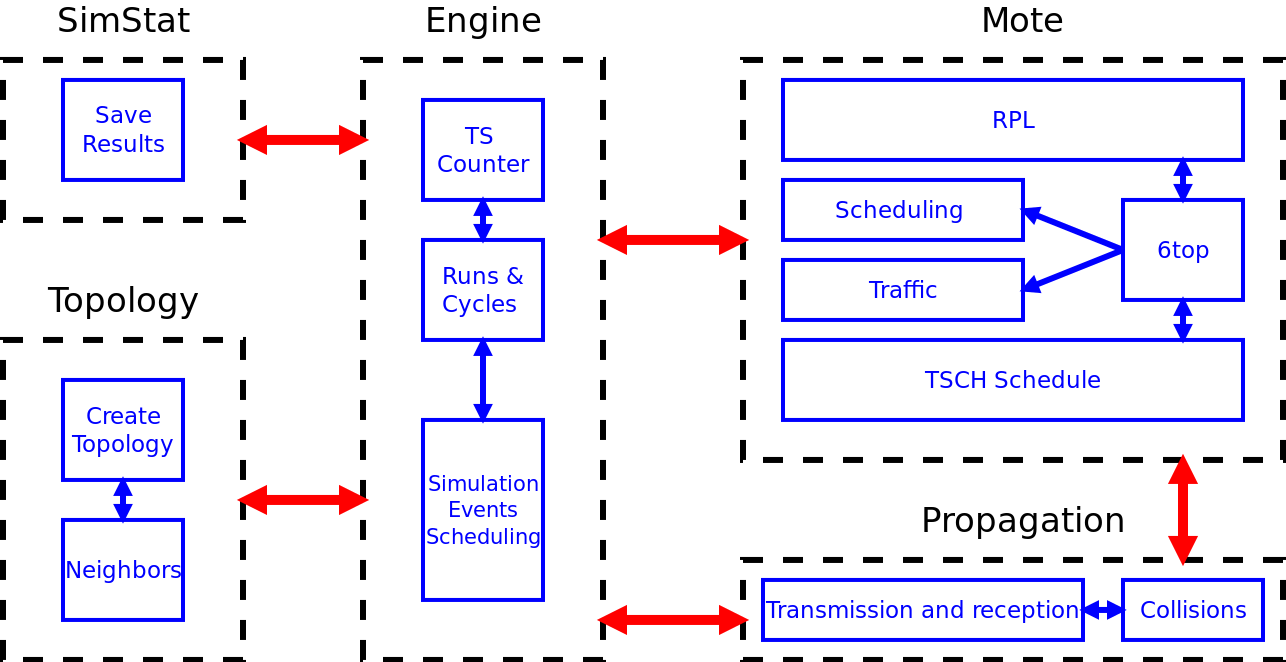
\includegraphics[width=\linewidth]{figures/SIM.png}

\end{figure}



\end{frame}
\end{withoutheadline}

\begin{withoutheadline}
\begin{frame}{Simulation Parameters}


\setbeamercolor{block title}{bg=blue!30,fg=black}
\setbeamercolor{block body}{bg=blue!10,fg=black}
\setbeamertemplate{blocks}[rounded][shadow=false]

\begin{center}
\begin{tabular}{l*{1}{c}r}
Parameter              & Value  \\
\hline
Number of Motes & $100$ \\
Number of cycles per run     & $1000$ \\
Number of runs per simulation     & $1000$ \\
Timeslot duration    & $10ms$ \\
Slotframe length     & $101$\\
Number of channels   & $16$ \\
Area            & $1Km\times1Km$ \\
Topology constraint     & $\geq$ 3 neighbors with PDR $50\,\%$ \\
Radio sensitivity           & $-97$ dBm \\
Radio range     & 100m \\
Traffic & 1 packet/node each 10 cycles 
\end{tabular}
%\captionof{table}{Simulator Parameters} \label{tab:para} 
\end{center}





\end{frame}
\end{withoutheadline}


\subsection{ Results}
\addtocounter{framenumber}{-1}
\begin{withoutheadline}
\begin{frame}{Comparison with random scheduling}

\begin{figure}[p]

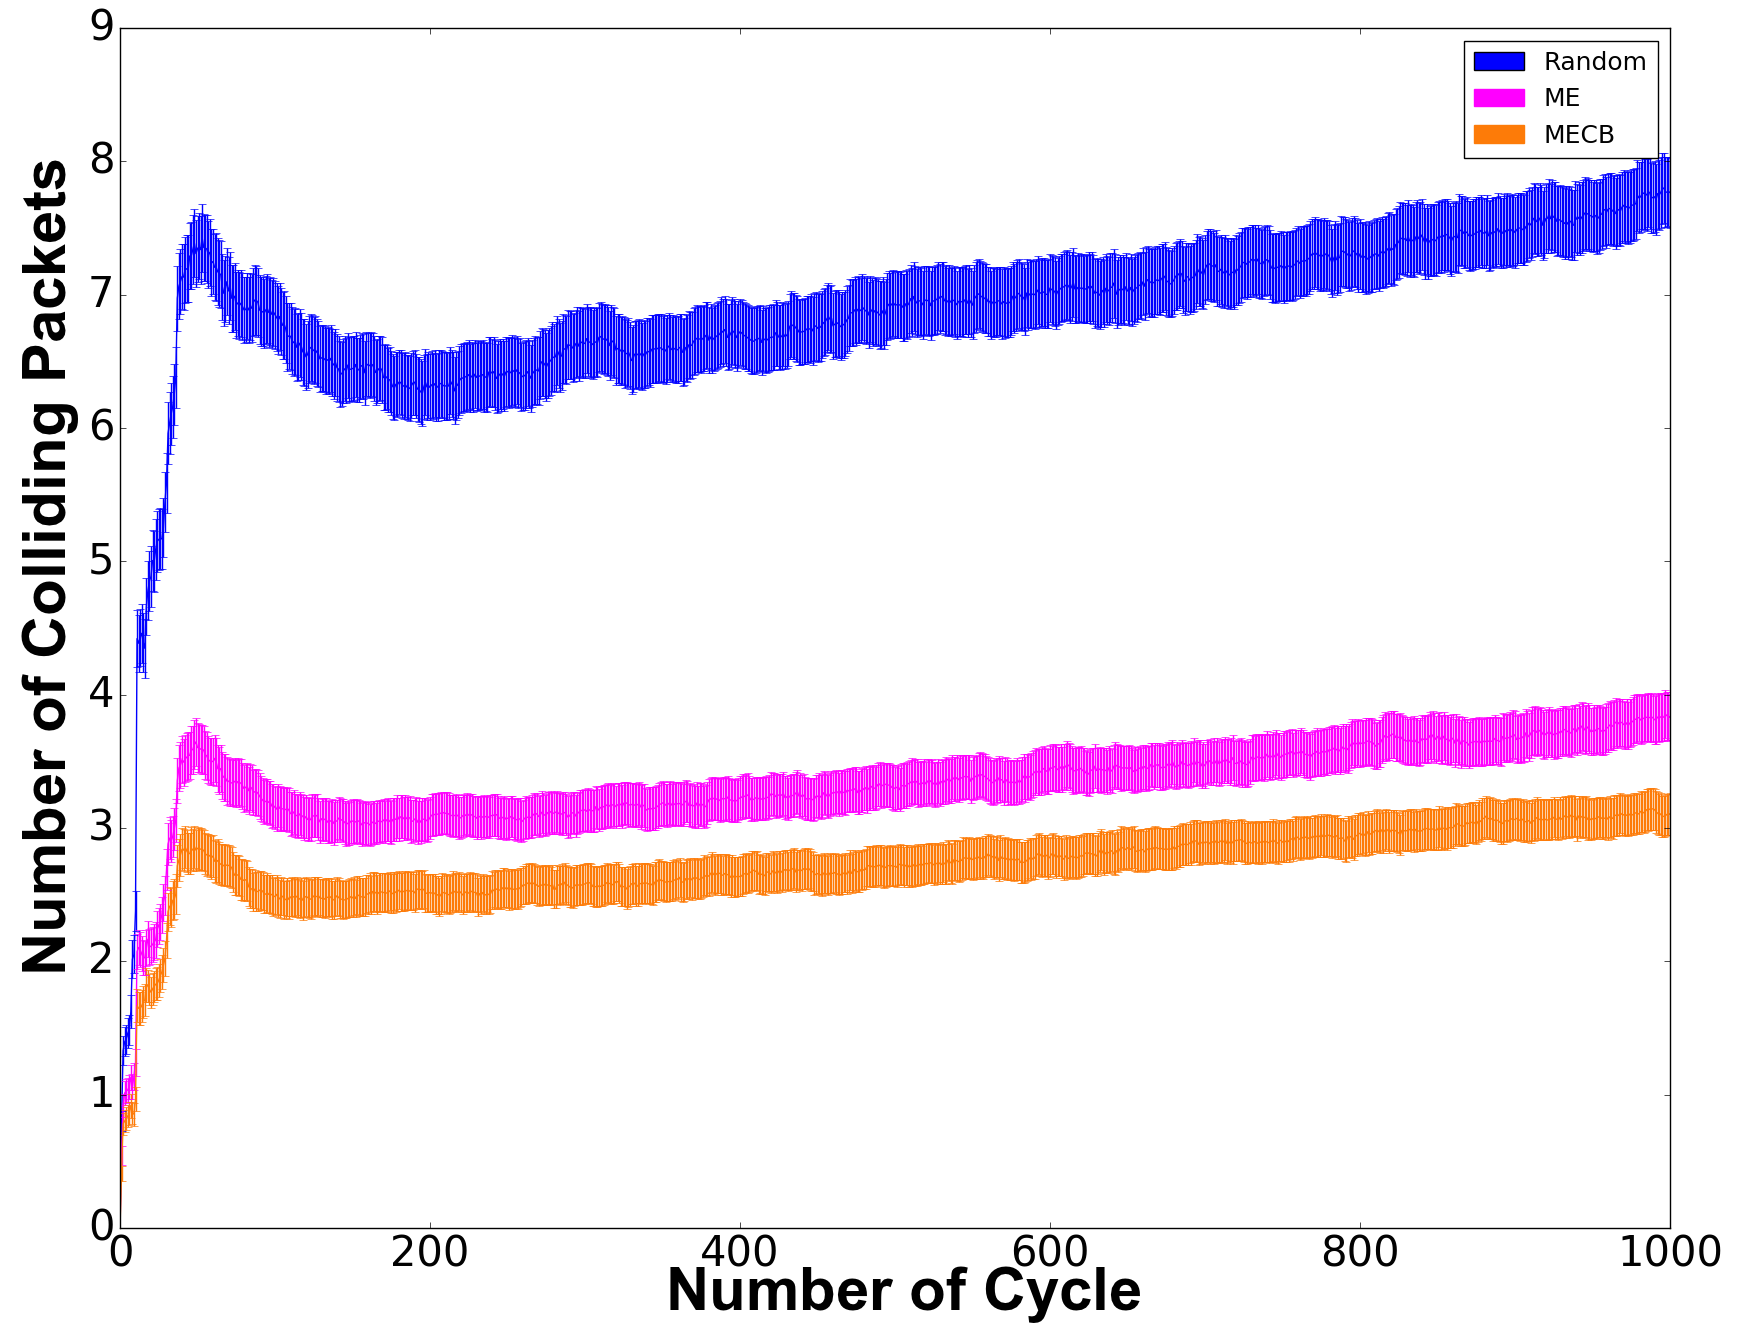
\includegraphics[width=\linewidth]{figures/graph1.png}

\end{figure}



\end{frame}
\end{withoutheadline}

\begin{withoutheadline}
\addtocounter{framenumber}{-1}
\begin{frame}{Comparison with random scheduling}

\begin{figure}[p]


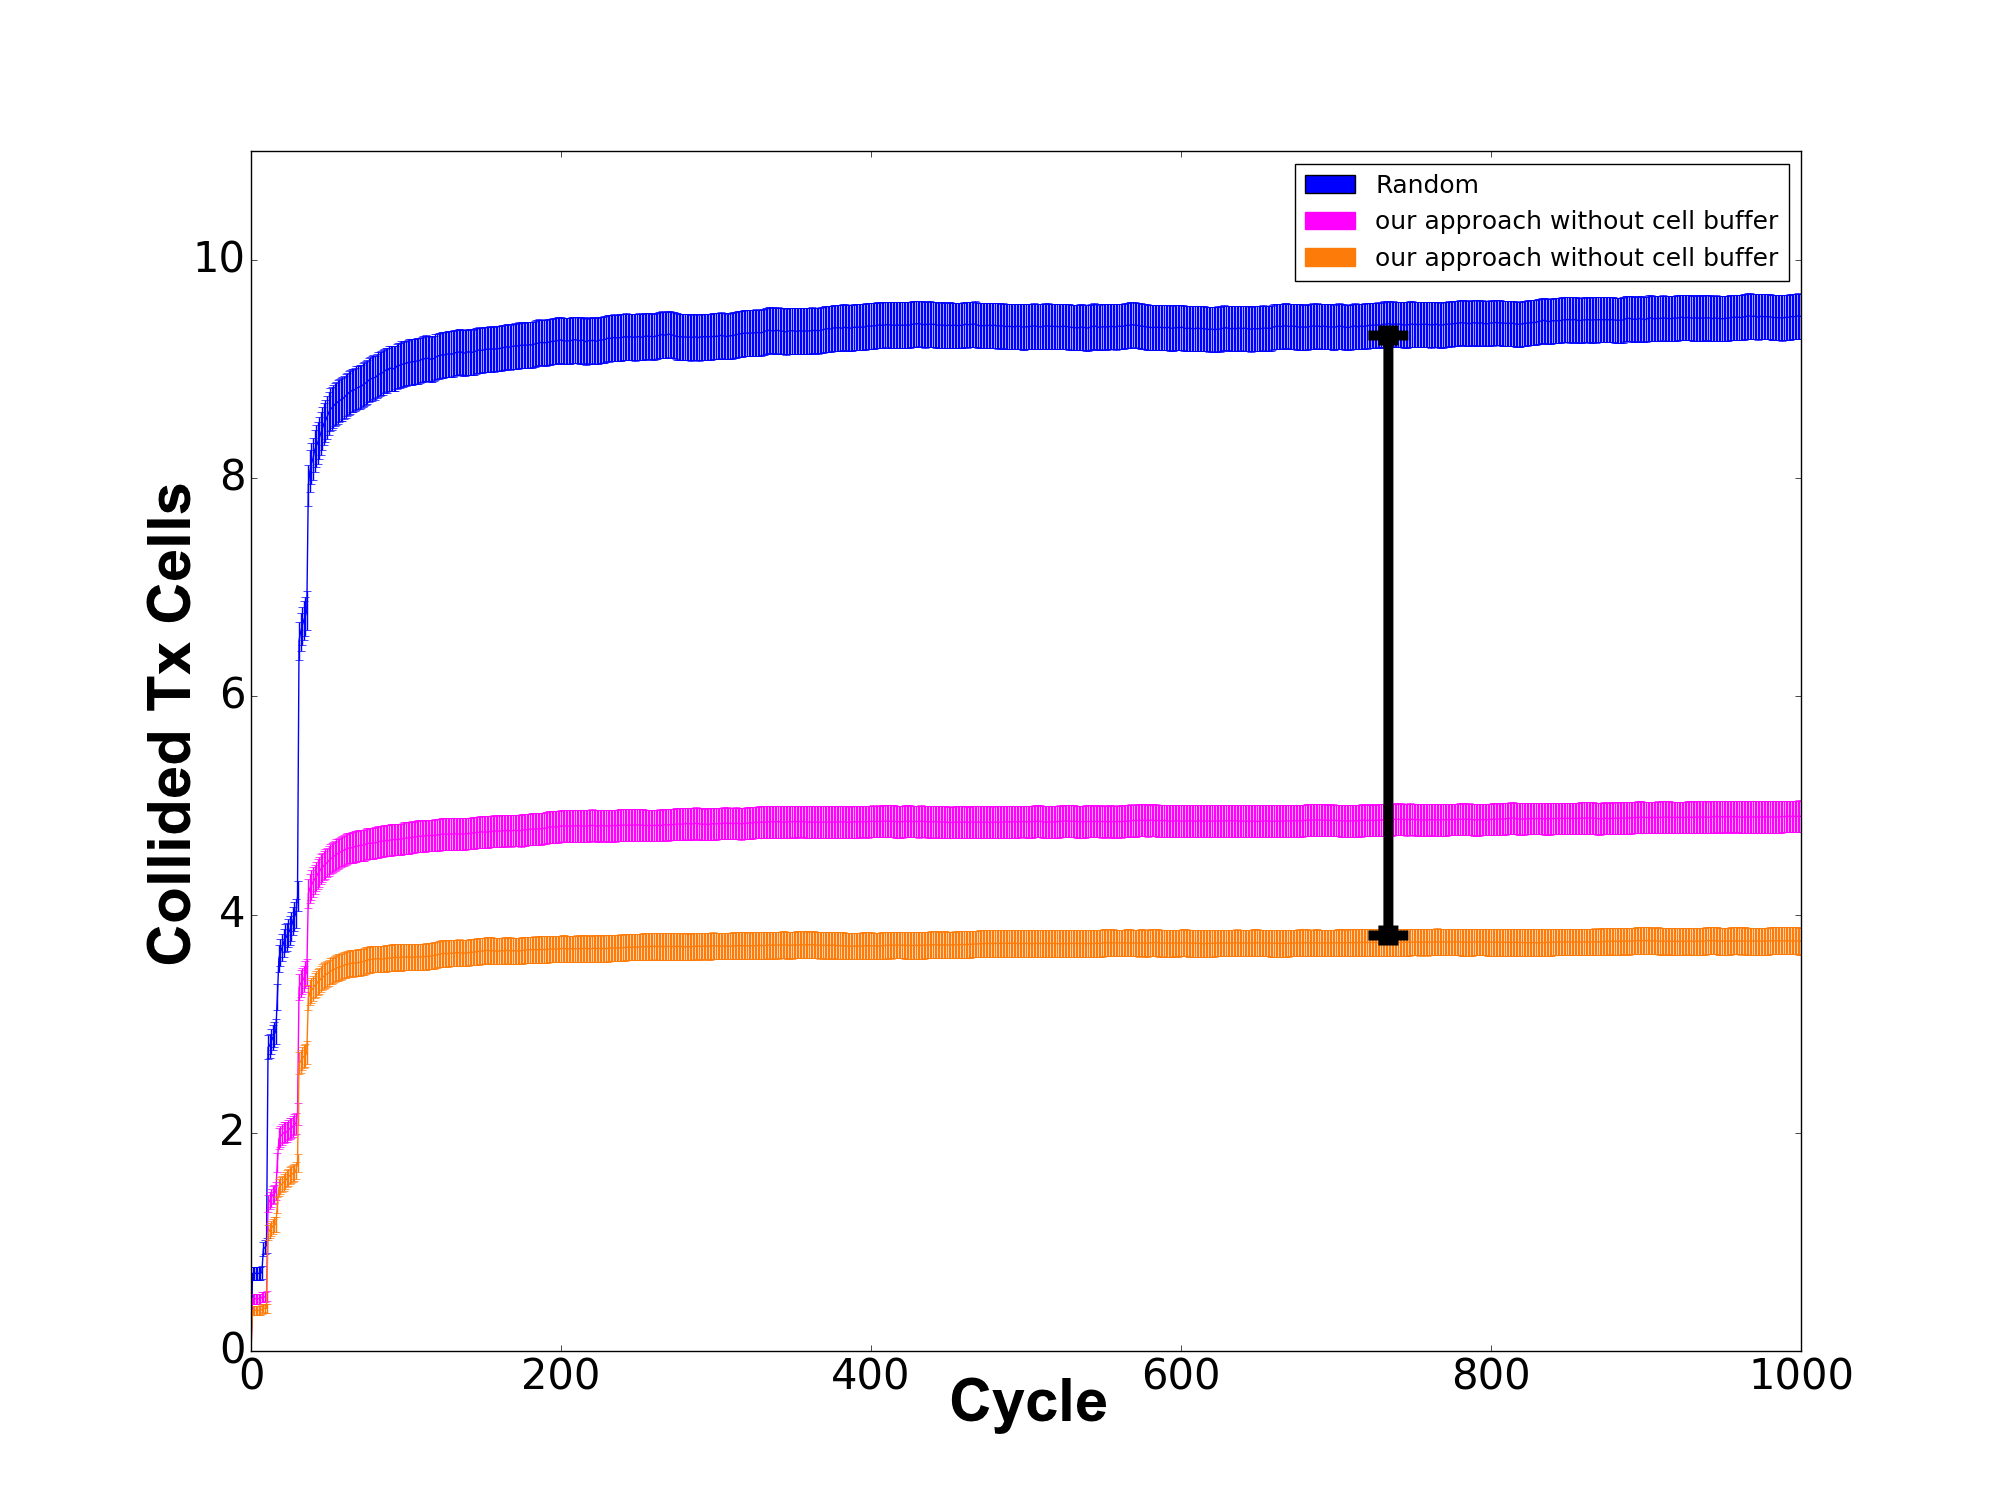
\includegraphics[width=\linewidth]{figures/graph1-1.png}
\end{figure}



\end{frame}
\end{withoutheadline}

\begin{withoutheadline}
\addtocounter{framenumber}{-1}
\begin{frame}{Comparison with random scheduling}

\begin{figure}[p]


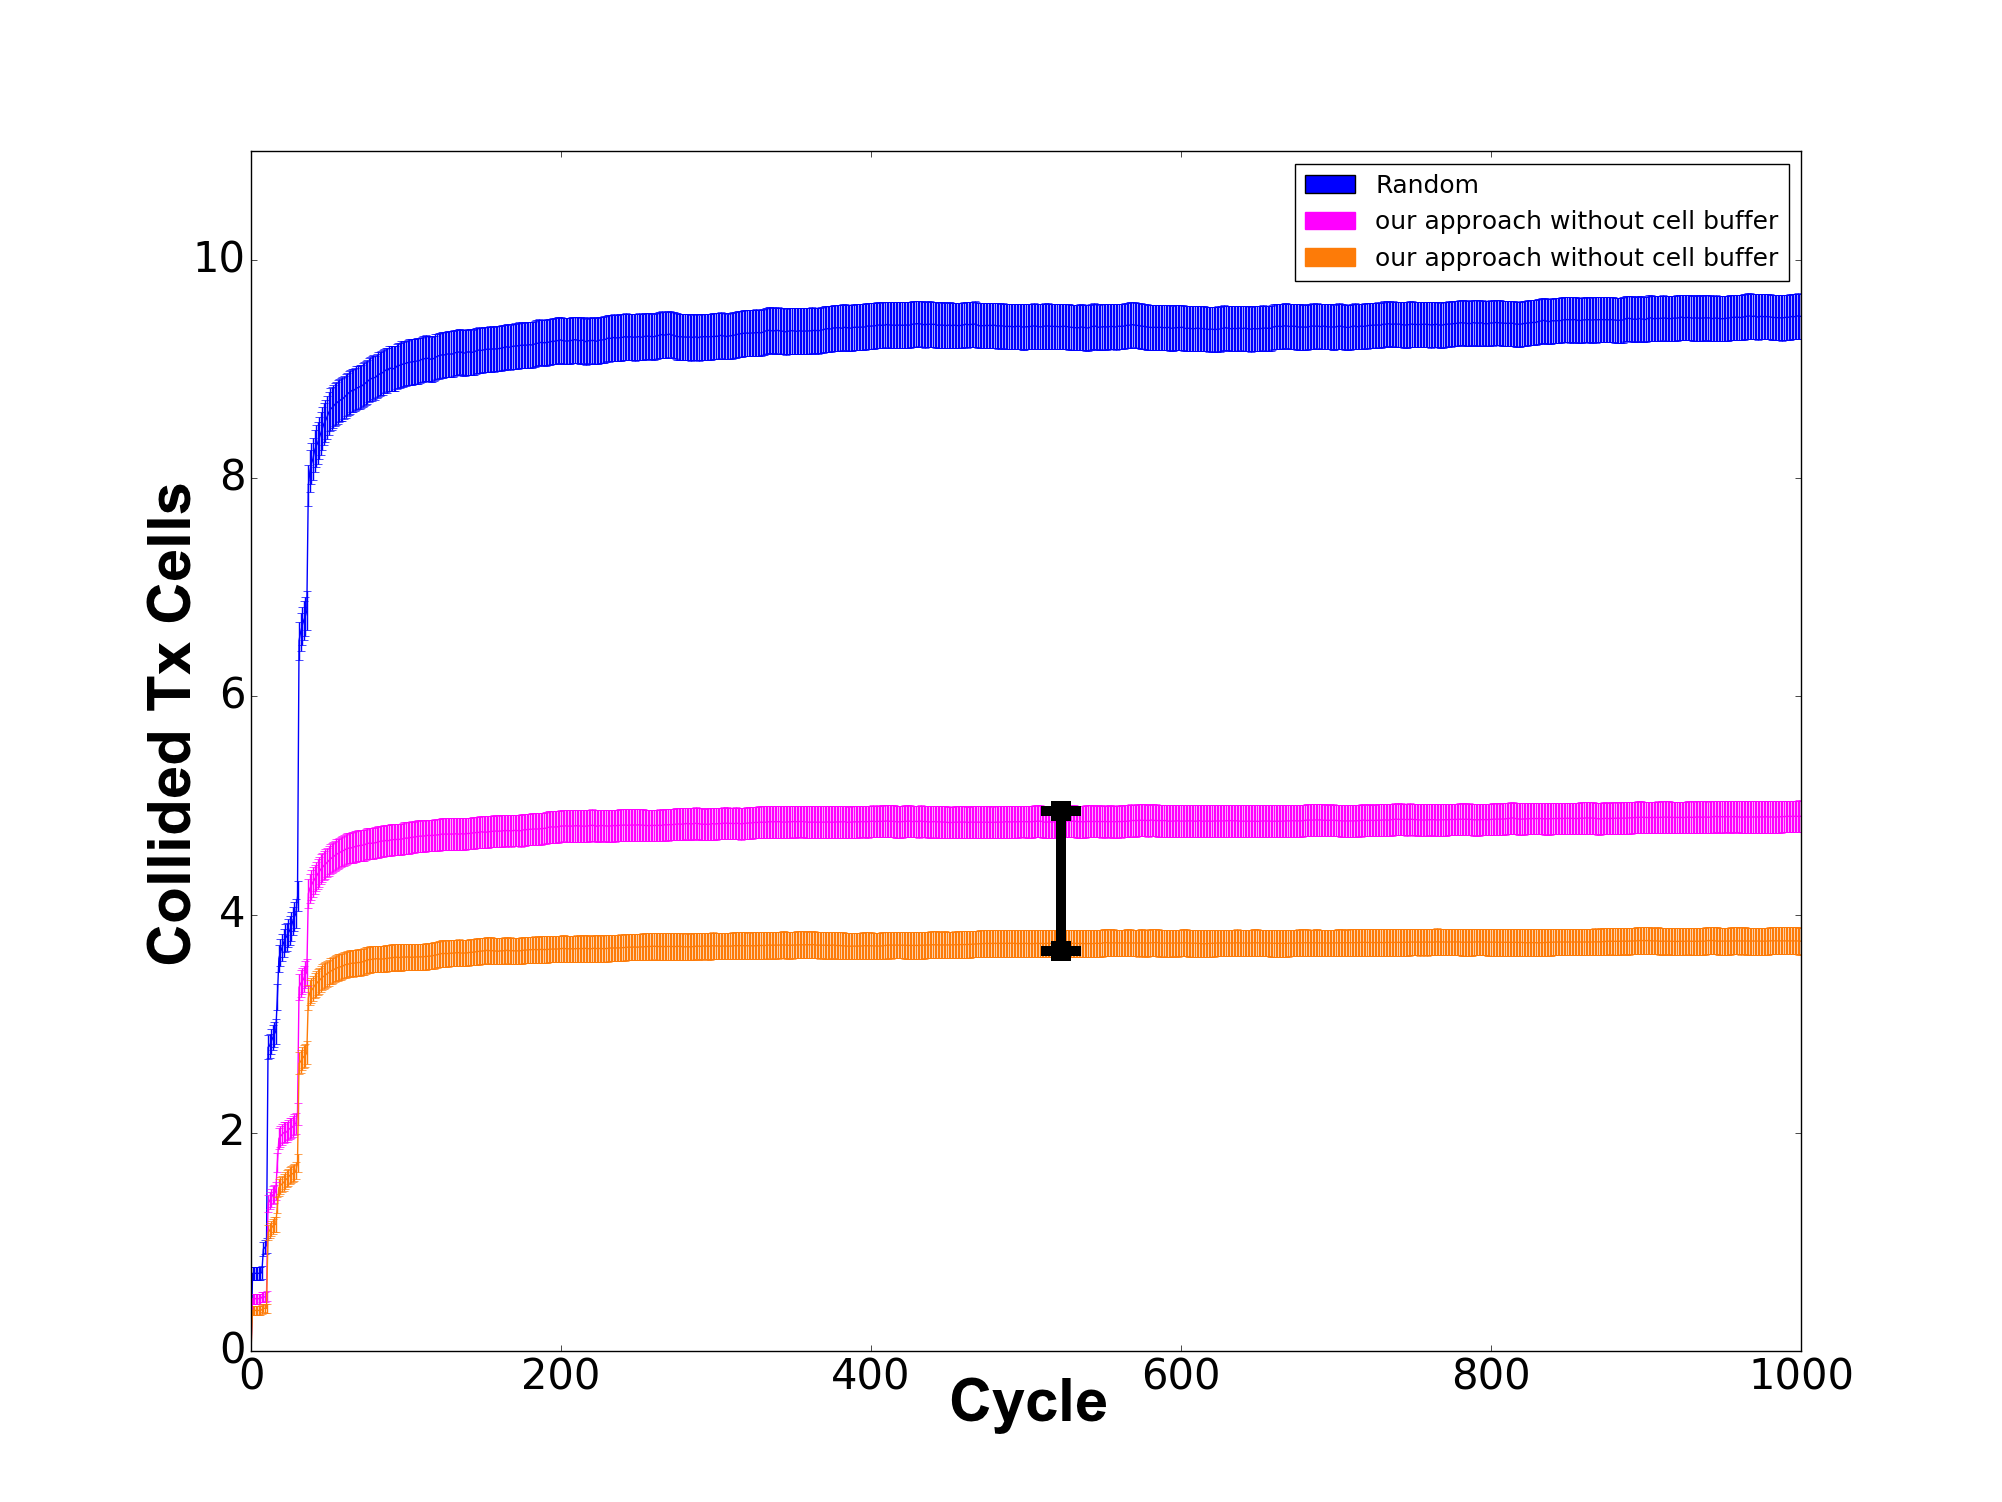
\includegraphics[width=\linewidth]{figures/graph1-2.png}
\end{figure}



\end{frame}
\end{withoutheadline}


\begin{withoutheadline}
\begin{frame}{ Results}


\setbeamercolor{block title}{bg=blue!30,fg=black}
\setbeamercolor{block body}{bg=blue!10,fg=black}
\setbeamertemplate{blocks}[rounded][shadow=false]


\begin{block}{Collision reasons}

    \begin{itemize}
    \item The lost 6top transactions. 
\item Special Case That Induce Collisions.
    
     
    
    \end{itemize}
    \end{block}

\centering
\begin{figure}[p]

\item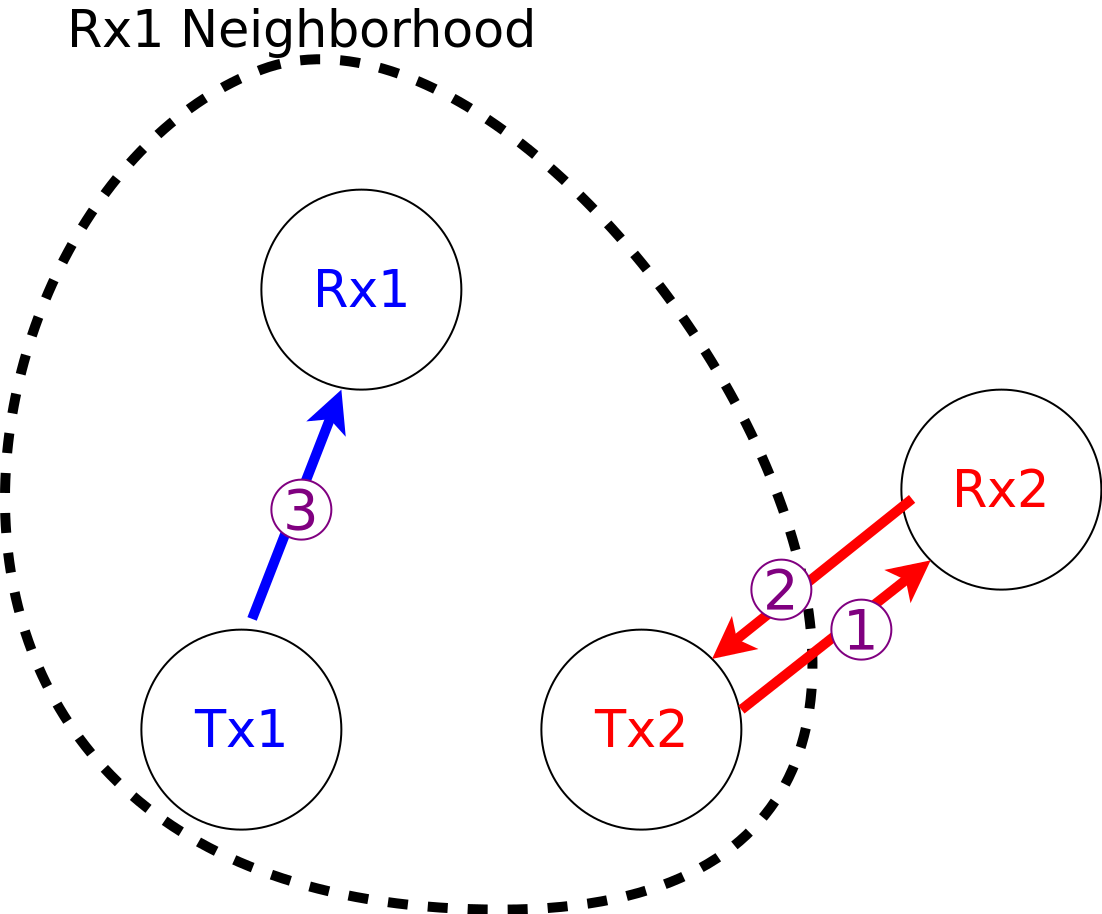
\includegraphics[width=0.4\linewidth]{figures/pro.png}
\end{figure}

\end{frame}
\end{withoutheadline}


\begin{withoutheadline}
\begin{frame}{Housekeeping Approach}


\setbeamercolor{block title}{bg=blue!30,fg=black}
\setbeamercolor{block body}{bg=blue!10,fg=black}
\setbeamertemplate{blocks}[rounded][shadow=false]
\begin{minipage}[t]{0.48\linewidth}

\begin{block}{Collision in Dedicated Cells}
    \begin{itemize}
    \item Housekeeping approach and cell relocation.
    \item Tx housekeeping. 
    \item<4-> Rx housekeeping. 
    \item<6-> Dealing with collisions after they occur. Good idea ?
    
    \end{itemize}
    \end{block}
\end{minipage}\hfill
\begin{minipage}[t]{0.48\linewidth}
\begin{figure}[p]
 \only<1>{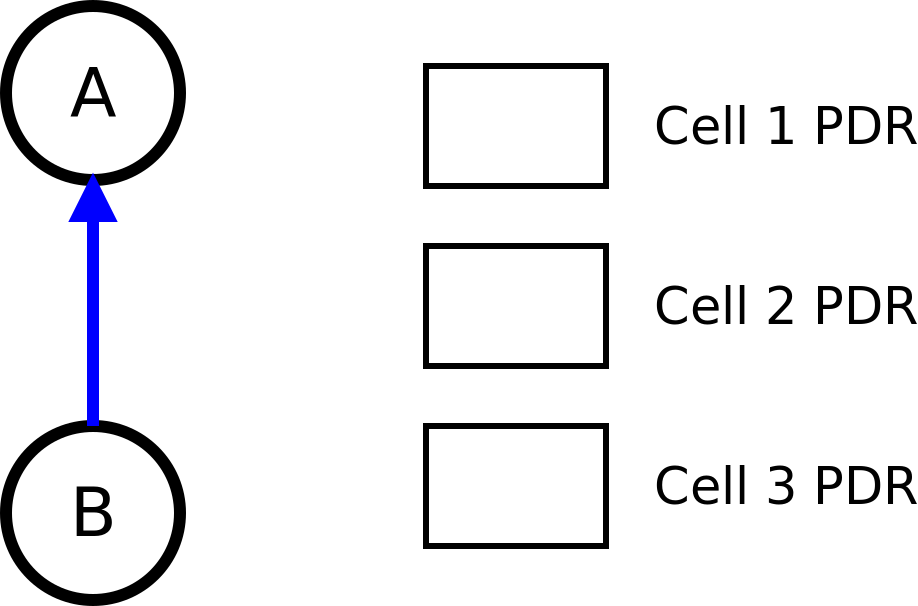
\includegraphics[width=\linewidth]{figures/hk1.png}}
 \only<2>{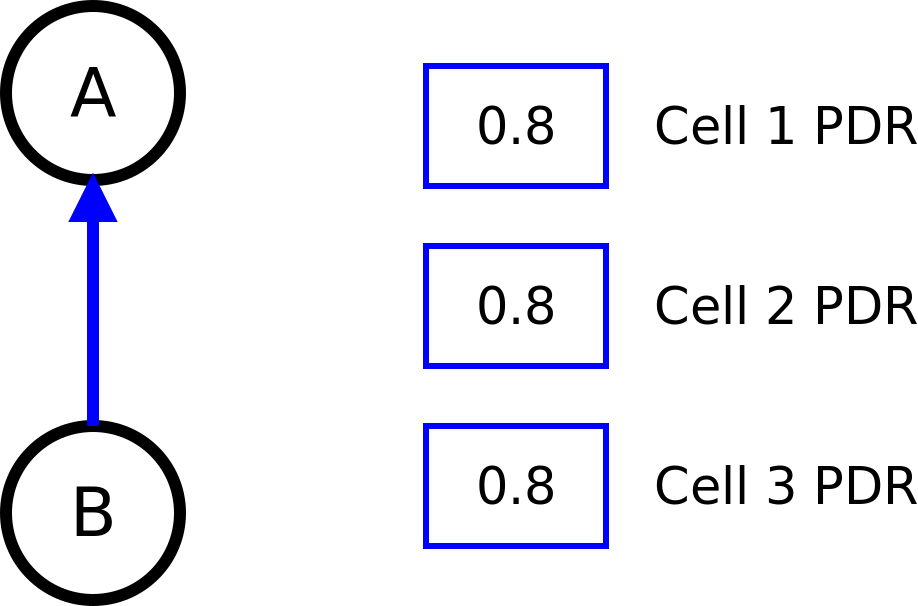
\includegraphics[width=\linewidth]{figures/hk2.png}}
  \only<3>{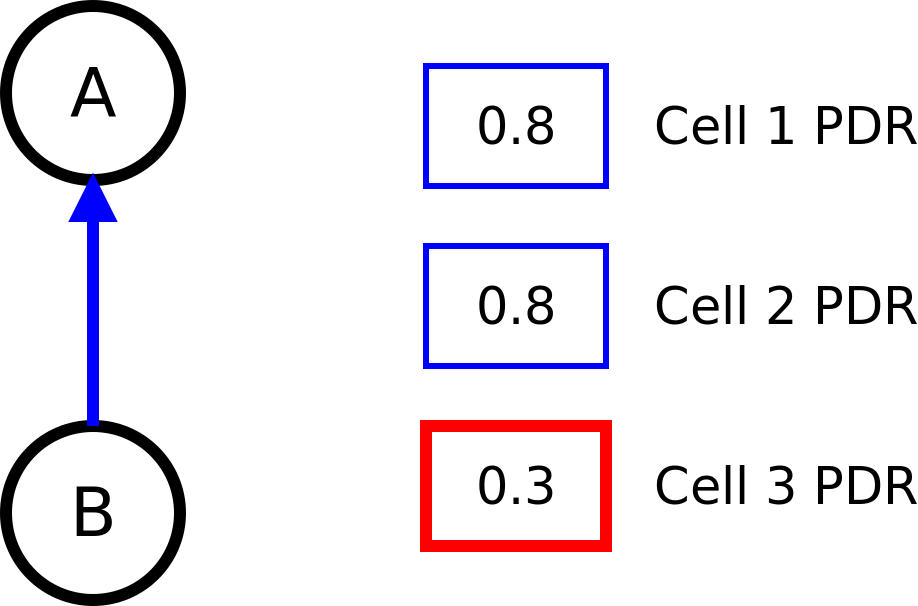
\includegraphics[width=\linewidth]{figures/hk3.png}}
  \only<4>{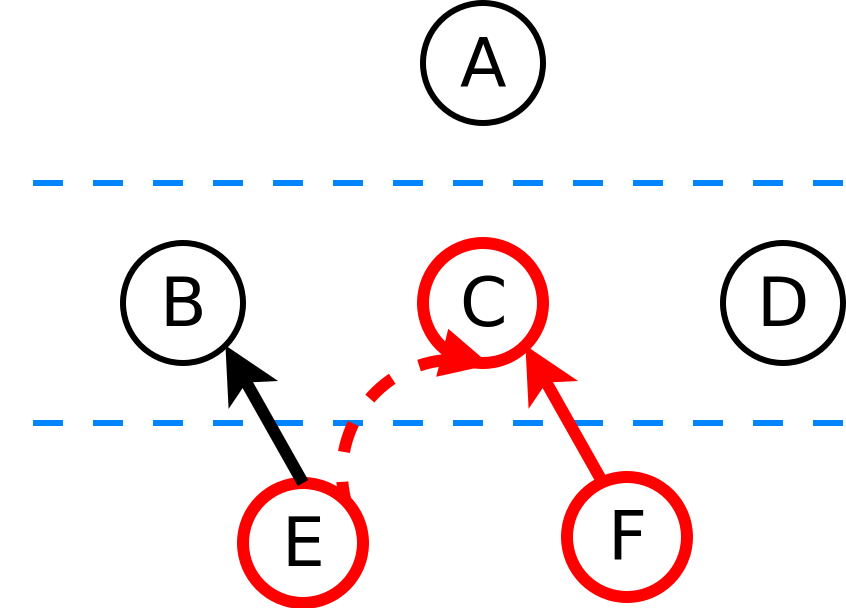
\includegraphics[width=\linewidth]{figures/rx1.png}}
  \only<5->{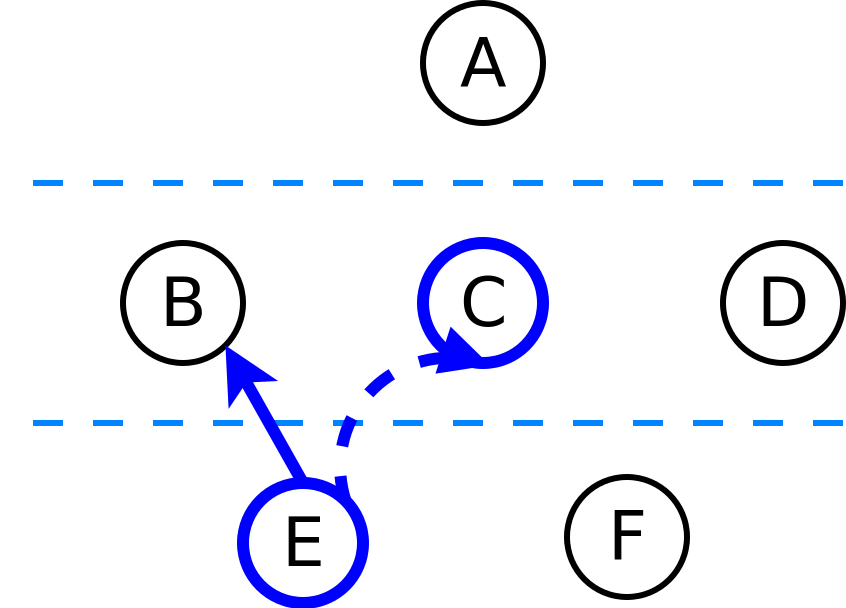
\includegraphics[width=\linewidth]{figures/rx2.png}}
  
\end{figure}
\end{minipage}

\end{frame}
\end{withoutheadline}


\begin{withoutheadline}
\begin{frame}{Comparison with Housekeeping }

\begin{figure}[p]

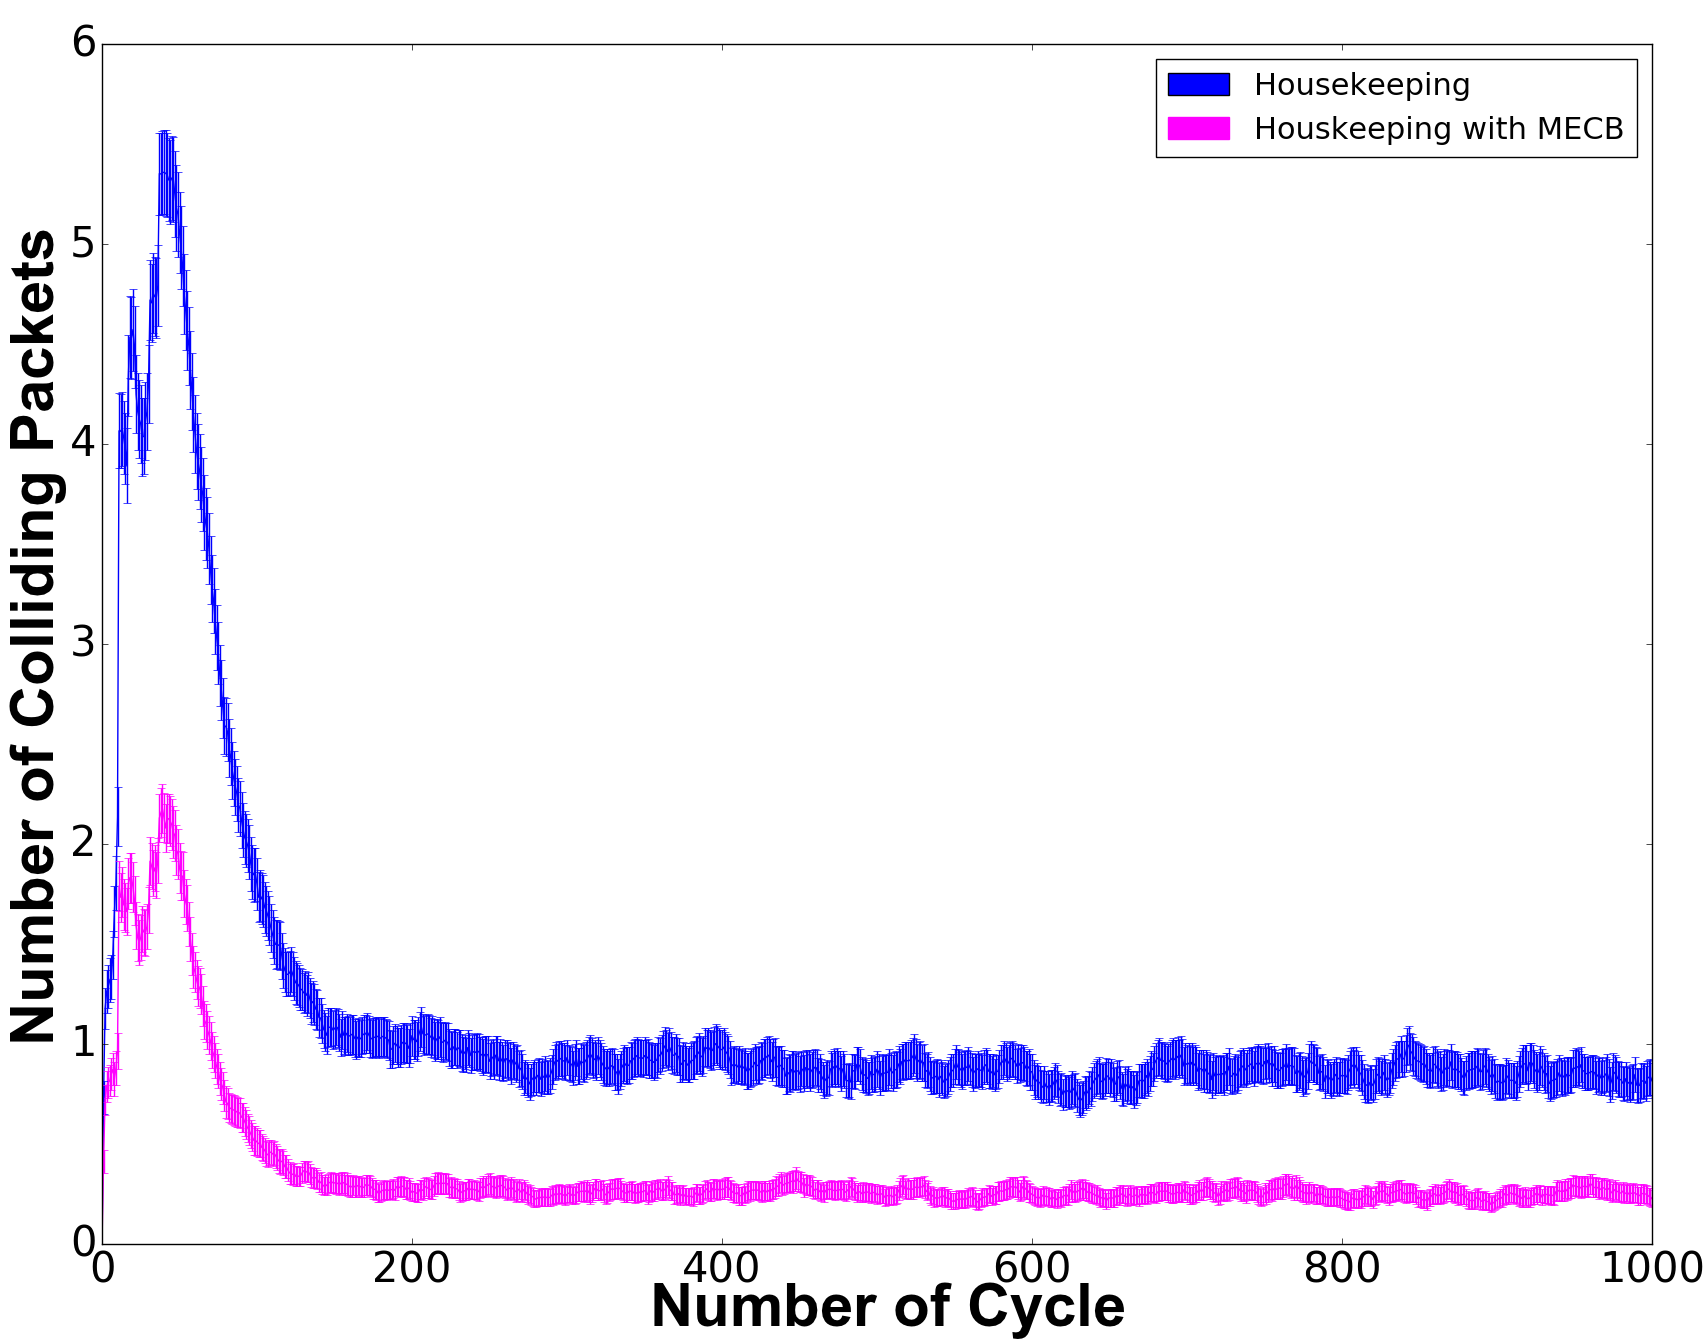
\includegraphics[width=\linewidth]{figures/graph2.png}
%\caption{Simulation of the Number of Collided Tx Cells as Function of Cycle Number (Time) - comparison with the housekeeping approach}
\end{figure}



\end{frame}
\end{withoutheadline}



%%%%%%%%%%%%%%%%%%%%%%%SUMMARY%%%%%%%%%%%%%%
\section{Summary and Contributions}

\begin{withoutheadline}
\begin{frame}{Summary}
  \begin{itemize}
  \item
    Our implementation introduce  \alert{no overhead } in the network.
  \item
    The implementation \alert{achieved 60\% reduction} in the number of collided Tx cells.
  \item The Combination of Our approach and Housekeeping accomplish an \alert{ almost collision free dedicated cells}.
  \end{itemize}
  
  \begin{itemize}
  \item
    Outlook
    \begin{itemize}
    \item
     Our goal is to reach a place were we have collision free network, using more complex methods.
    \item
      Our perspective in this project was work on 6top, but our next steps is to study the effects of traffic in the protocols performances.
    \end{itemize}
  \end{itemize}
\end{frame}
\end{withoutheadline}


\begin{withoutheadline}
\begin{frame}{Contributions}
  \begin{itemize}
  \item Understanding the simulator code.
  \item Optimizing, and implementing on top of this code.
  \item Designing the proposed mechanisms, and enhancing them.
  \item Publishing a poster in Computational sciences days in Grenoble, organized by LabEx PERSYVAL-Lab.
  \item Submitting a paper to Wimob 2017 conference. 
  \end{itemize}
  \begin{figure}[p]
\centering

\includegraphics[width=.5\linewidth]{figures/per.png}

\end{figure}
\end{frame}
\end{withoutheadline}

\section*{last}


\begin{withoutheadline}
\begin{frame}


\setbeamercolor{block title}{bg=blue!30,fg=black}
\setbeamercolor{block body}{bg=blue!10,fg=black}
\setbeamertemplate{blocks}[rounded][shadow=false]
\begin{tabular}{ccc}

\includegraphics[page=10, width=0.3\textwidth]{ali.pdf} &

\includegraphics[page=17, width=0.3\textwidth]{ali.pdf} &

\includegraphics[page=32, width=0.3\textwidth]{ali.pdf} \\


\includegraphics[page=35, width=0.3\textwidth]{ali.pdf} &

\includegraphics[page=42, width=0.3\textwidth]{ali.pdf} &

\includegraphics[page=46, width=0.3\textwidth]{ali.pdf} \\




\end{tabular}

\begin{block}{}
\centering Thanks for your attention!\\
Questions?
\end{block}


\end{frame}
\end{withoutheadline}
\appendix

\begin{withoutheadline}

\begin{frame}{IEEE802.15.4 Protocols}


\setbeamercolor{block title}{bg=blue!30,fg=black}
\setbeamercolor{block body}{bg=blue!10,fg=black}
\setbeamertemplate{blocks}[rounded][shadow=false]
\begin{minipage}[t]{0.48\linewidth}

\begin{block}{6TiSCH}
    \begin{itemize}
    \item  IEEE802.15.4 left the management of TSCH for other Protocols. 
    \item<2->  6TiSCH offered the integration of TSCH over IPv6.
    \item<3->  6TiSCH operation sublayer (6top) offered the management of TSCH:
             \begin{itemize}
             \item Centralized algorithm.
             \item<4-> Distributed algorithm. 
             \end{itemize}
    \item<5-> 6top contains:
     \begin{itemize}
             \item 6top transactions.
             \item<6-> Scheduling function. 
             \end{itemize}
    
    \end{itemize}
    \end{block}
\end{minipage}\hfill
\begin{minipage}[t]{0.48\linewidth}
\vskip 5em
\begin{figure}[p]

 \only<3>{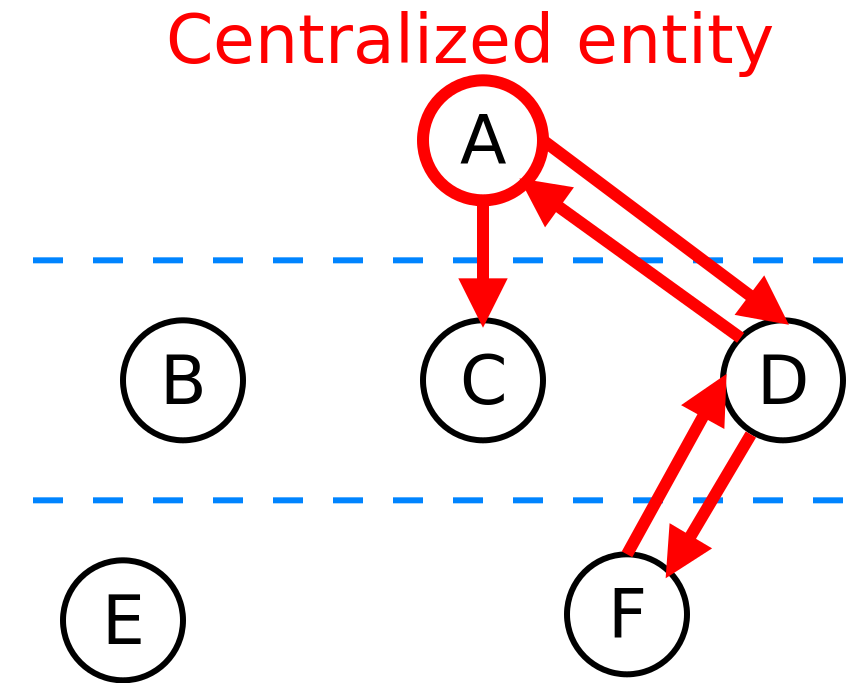
\includegraphics[width=\linewidth]{figures/Cent.png}}
  \only<4->{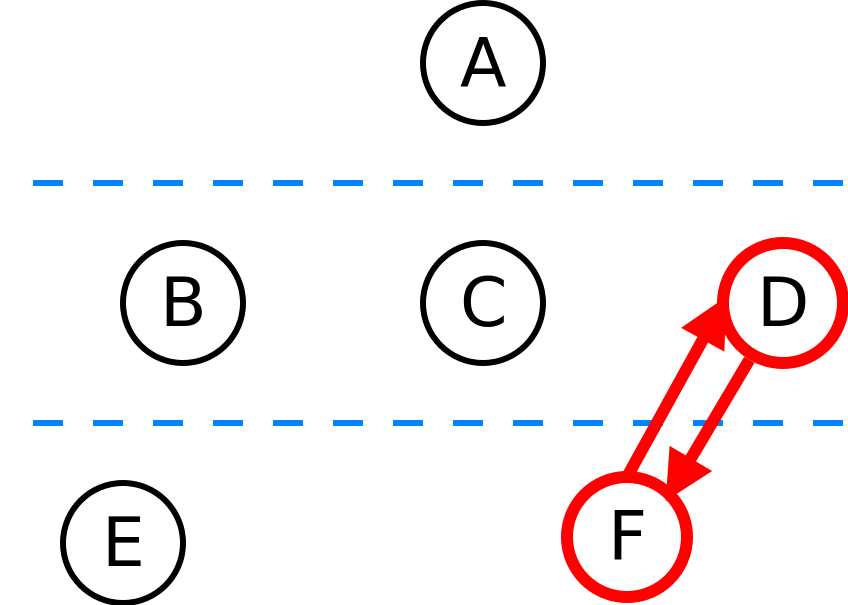
\includegraphics[width=\linewidth]{figures/Dist.png}}
  
\end{figure}

\end{minipage}
\end{frame}
\end{withoutheadline}

\end{document}


